\documentclass[12pt, twoside]{report}

% a4 paper
\usepackage[a4paper, margin = 30mm, bindingoffset = 6mm]{geometry}
%\usepackage[a4paper, margin = 30mm, bindingoffset = 6mm, showframe]{geometry}

% set 1.5 line spacing
\usepackage[onehalfspacing]{setspace}

% create header and footer
\usepackage{fancyhdr}

% main page style
\pagestyle{fancy}
\fancyhead{}
\fancyhead[RE,LO]{\nouppercase{\leftmark}}
\fancyfoot{}
\fancyfoot[C]{\thepage}

% chapter page style
\fancypagestyle{chapter} {
	\fancyhead{}
	\renewcommand{\headrulewidth}{0pt}
	\fancyfoot{}
	\fancyfoot[C]{\thepage}
}

% redefine chapter command
\makeatletter
    \let\stdchapter\chapter
    \renewcommand*\chapter{%
    \@ifstar{\starchapter}{\@dblarg\nostarchapter}}
    \newcommand*\starchapter[1]{%
        \stdchapter*{#1}
        \thispagestyle{chapter}
        \markboth{\MakeUppercase{#1}}{}
    }
    \def\nostarchapter[#1]#2{%
        \stdchapter[{#1}]{#2}
        \thispagestyle{chapter}
    }
\makeatother

% get warning to change head height for header
\setlength{\headheight}{14.5pt} 

% limit table of contents to chapters and sections
\setcounter{tocdepth}{1}

% can use [nosep] or [noitemsep] in itemize and enumerate to reduce line spacing between items
\usepackage[shortlabels]{enumitem}

% add bibliography
\usepackage[backend = bibtex, style = authoryear, sorting = ynt, natbib]{biblatex}
\addbibresource{bibliography.bib}

% add figures
\usepackage{graphicx}
\graphicspath{ {Figures/} }
\usepackage{subcaption}

% format for algorithms
\usepackage{algorithm}
\usepackage[noend]{algpseudocode}

% import packages
\usepackage{amssymb}
\usepackage{amsmath}
\usepackage{tabularx}
\usepackage{bbm}
\usepackage{multirow}
\usepackage{mathtools}

% empty page
\newcommand*\emptypage{
    \newpage
    \null
    \thispagestyle{empty}
    \newpage
}

% define argmin and argmax
\DeclareMathOperator*{\argmin}{arg\,min}
\DeclareMathOperator*{\argmax}{arg\,max}

\begin{document}

\begin{titlepage}
    \begin{center}
        \vspace*{1cm}
        
        \Huge
        \textbf{Queues with a Dynamic Schedule}
        
        \vspace{0.5cm}
        
        \LARGE
        John Gilbertson
        
        \vfill
        
        A thesis presented for the degree of\\
        Master of Science (Mathematics and Statistics)
        
        \vspace{0.8cm}
        
        \Large
        Supervised by Professor Peter Taylor\\
        Department of Mathematics and Statistics\\
        The University of Melbourne\\
        October 2016
        
    \end{center}
\end{titlepage}
















































\emptypage

\chapter*{Declaration}

This thesis is the sole work of the author whose name appears on the title page and it contains no material which the author has previously submitted for assessment at the University of Melbourne or elsewhere. To the best of my knowledge and belief, the thesis contains no material previously published or written by another person, in the form of unacknowledged quotations or mathematical workings or in any other form, except where due reference is made. I declare that I have read, and in undertaking this research I have complied with, the University's Code of Conduct for Research. I also declare that I understand what is meant by plagiarism and that this is unacceptable.

\vspace{1cm}

\noindent{}Signed

\vspace{0.5cm}

\hspace{1.5cm} John Gilbertson

\newpage

\emptypage

\chapter*{Abstract}

Queues with scheduled arrivals occur frequently in society, most notably in health care. These are queues where customer arrival times are scheduled in advance. In this thesis, we study both static and dynamic schedules. A static schedule is fixed for the duration of service whereas a dynamic schedule is chosen progressively during service. Dynamic schedules reflect the ability of a scheduler to reschedule customer arrival times during service. In this thesis, we compare the two schedules both in terms of expected behaviour and through use of a simulation study.

\emptypage

\tableofcontents

\chapter{Introduction}

Introduction goes here.

\chapter{Literature Review}
Queues with scheduled arrivals are widely studied. There is a large body of literature studying the potential of appointment systems to reduce customer waiting times and waiting room congestion. This research is essential as health care providers in particular are under a great deal of pressure to improve service quality and efficiency \citep{Goldsmith}.  Before we explore the detail of this thesis, it is important to review some of the papers that study this problem.

\citet{Fomundam}, and \citet{Cayirli} provide comprehensive surveys of research on appointment scheduling. Most of the papers on scheduled arrivals can be classed into two categories. Those that design algorithms to determine schedules, and those that evaluate schedules using simulation. While simulation studies can easily model complicated customer flows, queuing models often provide more generic results than simulation \citep{Green}.

The foundation paper on modeling queues with scheduled arrivals is \citet{Bailey}. Bailey proposes that customers' waiting times can be reduced without a significant increase in the server's idle time. The Bailey rule, which is commonly referenced in literature, is that customers should be scheduled to arrive at fixed intervals with two customers scheduled to arrive at the start of service. Bailey uses random numbers to run off a series of independent service times. Bailey finds that a great deal of time wasted by customers can be reduced without a significant increase in the server's idle time. Under the Bailey rule, customers with late appointments will wait longer than those with early appointments. This lack of uniformity might be perceived as unfair and thus an undesirable property of a schedule. 

\citet{Pegden} extend Bailey's paper. They present an algorithm to iteratively determine the optimal arrival times for $n$ customers that need to be scheduled. The optimal arrival times are those that minimise a weighted sum of the expected customers' waiting time and the expected server's total availability time.

Pegden and Rosenshine prove that their objective function is convex for $n \leq 4$, thus their algorithm finds the optimal schedule. While they conjecture that the objective function is convex for all $n$, it has not been proven. Nevertheless, we refer to the times returned by their algorithm as `optimal times' throughout this thesis. This is both for simplicity and because we believe that they are in fact optimal.

\citet{Stein} apply Pegden and Roshenshine's model to obtain numerical results for situations with more than three customers. The optimal times between successive customers become near constant as $n$ grows. This is the often observed dome-shape. Figure~\ref{fig:Lit_Dome_Shape} plots several examples of this dome shape. Optimal interarrival times exhibit a common pattern where they initially increase towards the middle of a session, and then decrease. This figure will be explained more clearly in Chapter~\ref{chap:Static}.
\begin{figure}[htb]
	\centering
	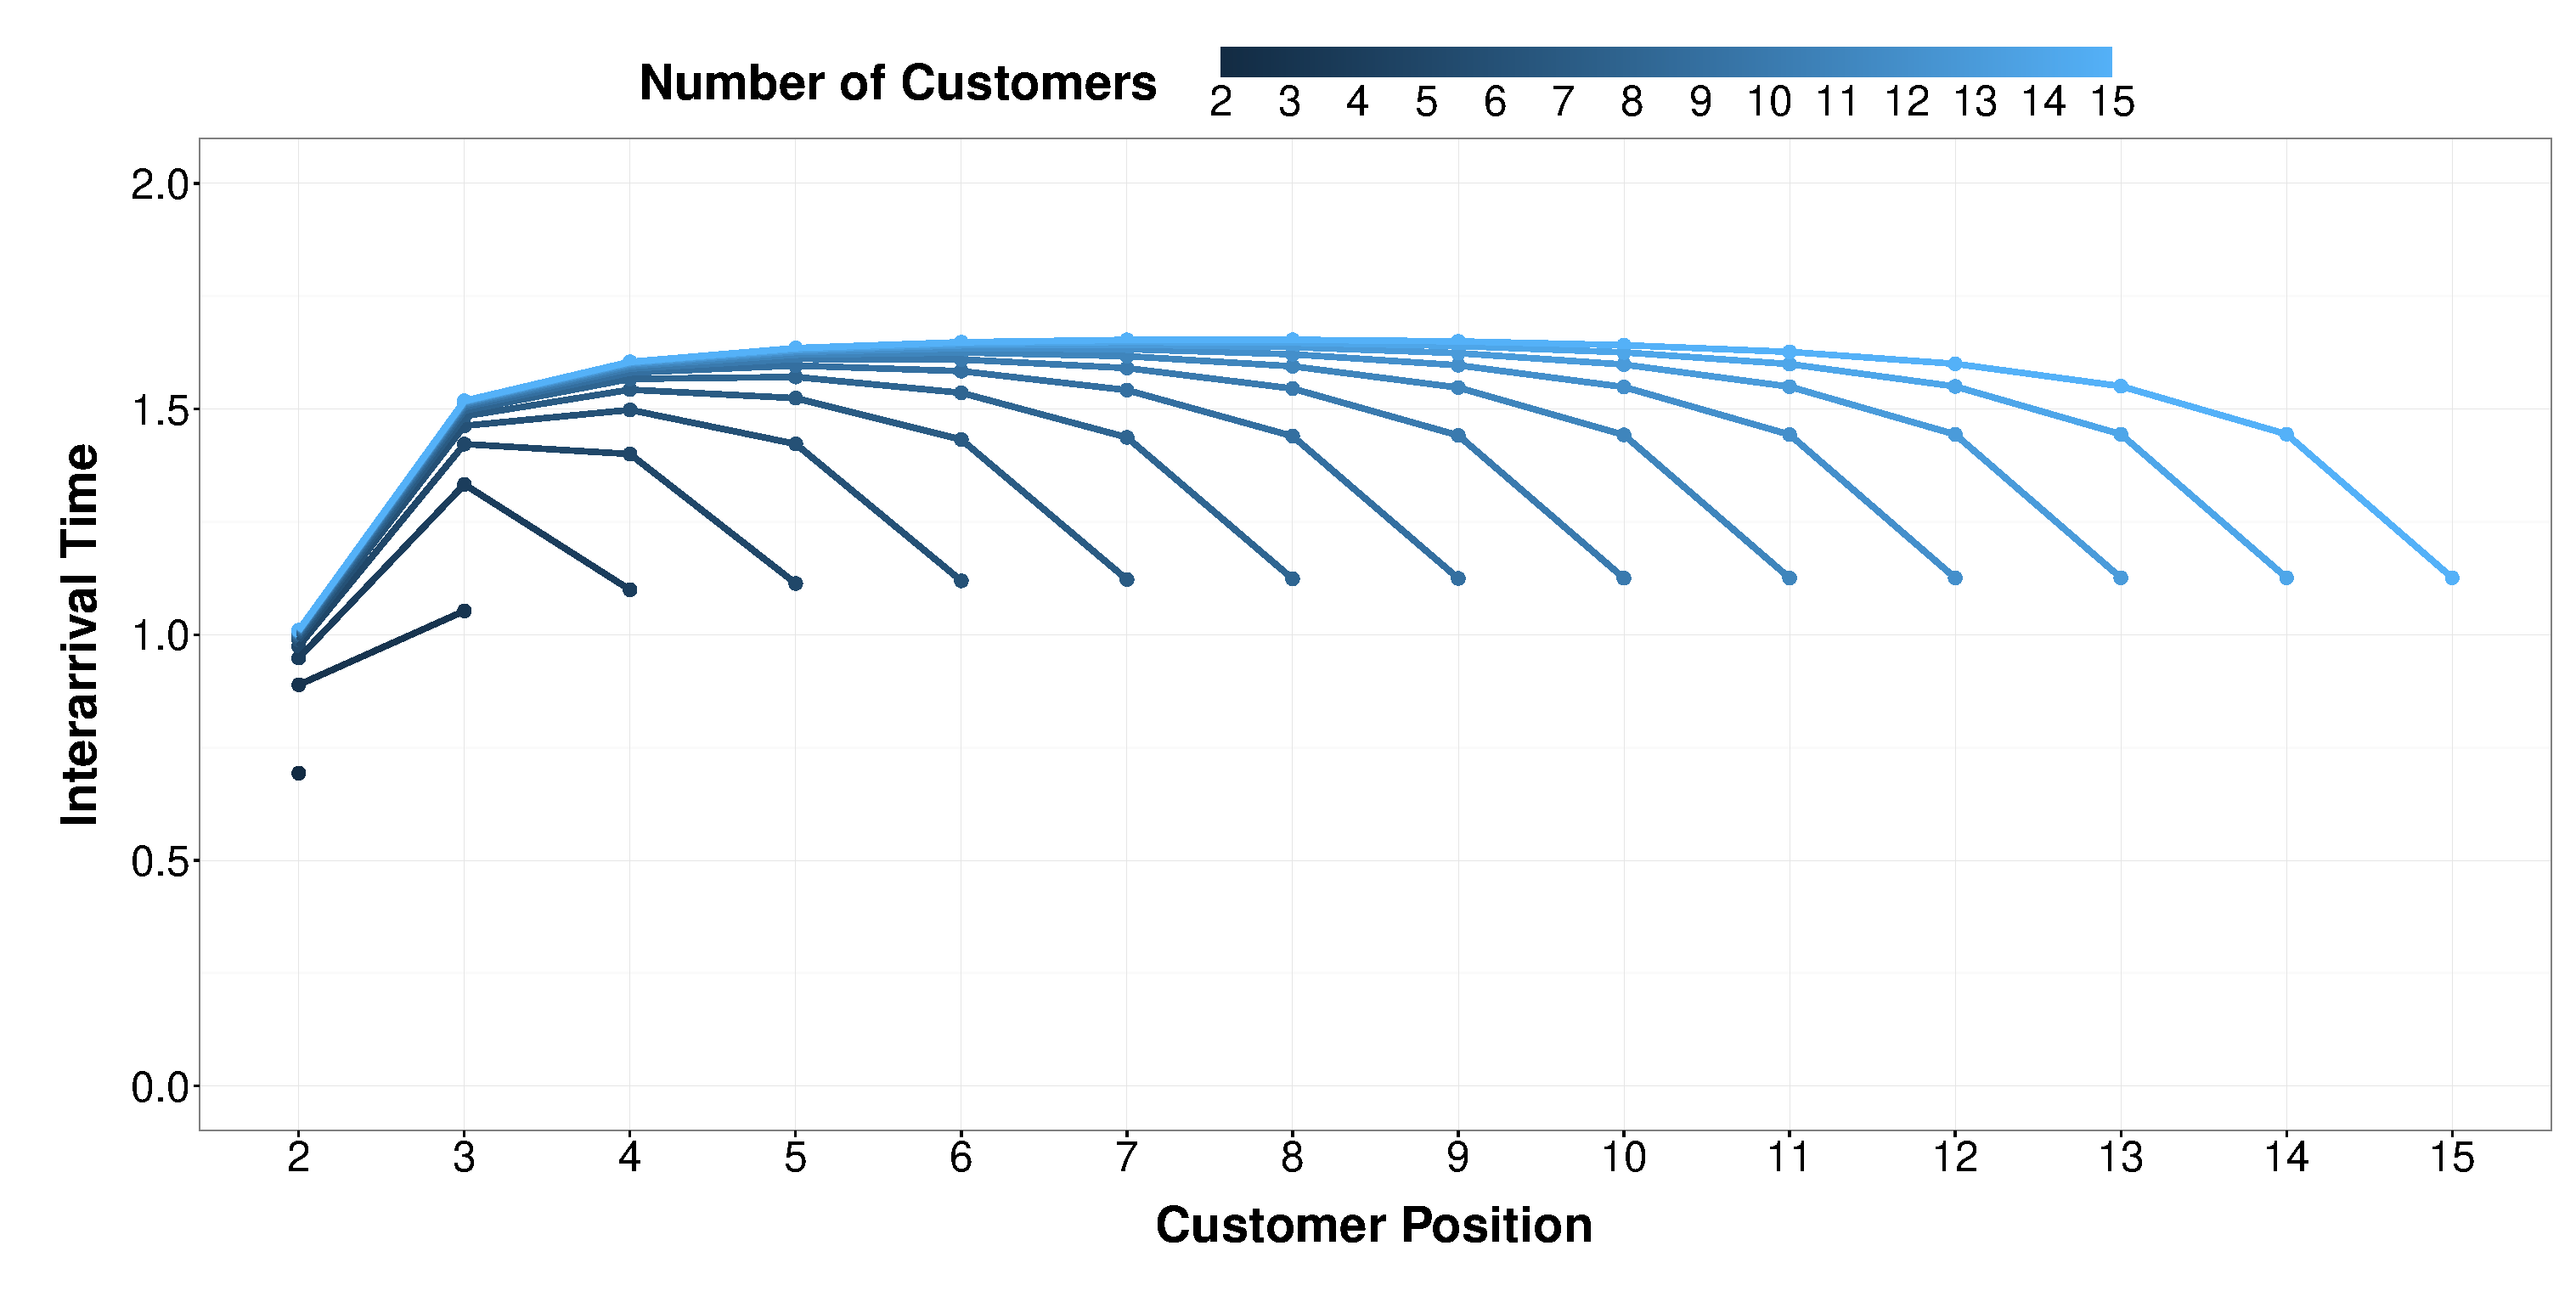
\includegraphics[width = 0.85\textwidth]{Static_Line_Interarrival_Num.eps}
	\caption{Optimal interarrival time for each customer after the first customer showing the dome-shapes as found by \citet{Stein}. Figure is explained more clearly in Chapter~\ref{chap:Static}. Figure generated assuming $\mu = 1$ and $\gamma = 0.5$. Each line is plotted for a given number of customers ($n$). The lightest line is the optimal schedule for $15$ customers. As $n$ decreases, the lines become darker.}
	\label{fig:Lit_Dome_Shape}
\end{figure}

Stein and C\^{o}te simplify their model by requiring the intervals between arriving customers to be constant. This commonly studied restriction makes the model more easily applicable in practice, and more computationally efficient to solve for a large number of customers.

Stein and C\^{o}te apply queuing theory results to solve the model for the optimal arrival interval assuming the queue reaches its steady state distribution. This assumption greatly reduces the computation required. However, in practice, it is common to find services that never reach steady state. \citet{Babes} attempt to apply steady state queuing theory, but find their results tend to be very different from those observed in real operation.

These key papers by Bailey, Pegden and Rosenshine, and Stein and C\^{o}te provide the basis for a more realistic exploration of health care systems. \citet{Delaurentis} highlight that customer no-shows can lead to a waste of resources. \citet{Mendel} incorporates the probability of a customer not showing up into the model presented by Pegden and Rosenshine. Unsurprisingly, no-shows lead to lower expected waiting times for customers who do show up.

The presence of walk-ins (regular and emergency) can disrupt a schedule. \citet{Gupta} propose a system where non-routine requests are superimposed on top of routine scheduled requests. \citet{Fiems} investigate the effect of emergency requests on the waiting times of scheduled customers. Fiems et al. model a system with deterministic service times and discrete time. Despite this research, Cayirli and Veral suggest that walk-ins are neglected in most studies. Further research could investigate their effect on optimal arrival times.

\citet{Mondschein} observe that the majority of the literature assumes that demand is exogenous and independent of customers' waiting times. These papers assume the total number of customers is fixed and independent of waiting times. The vast majority of servers are now private (including medical servers), so face competitive environments. Mondschein and Weintraub thus present a model where demand depends on the customers' expected waiting time.

Few authors attempt to model a dynamic schedule. \citet{Wang} considers the problem of scheduling a new customer when there are already a number of customers with fixed scheduled arrival times. The aim is to determine the optimal arrival time for the new customer such that the objective function remains optimal. However, Wang is criticised for not having a truly dynamic model \citep{Erdogan}. The initial scheduling of the customers ignores the possibility of an additional customer needing to be scheduled.

Simulation is a useful tool to analyse the effectiveness of appointment policies. \citet{Kao} use simulation to compliment their results obtained from queuing theory. \citet{Ho} study the performance of eight different appointment rules under different scenarios. They find that no rule will perform well under all circumstances.

Case studies can test the real world applications of an appointment system. While they lack generalisation, they are necessary to compliment the theoretical research. \citet{Rockart} show individual block systems lead to more punctual doctors and patients, and less no-shows. \citet{Walter} indicates that the simple grouping of inpatients and outpatients results in a substantial reduction in the doctor's idle time.

Unfortunately, \citet{Cayirli} lament that despite much published work, the impact of appointment systems on outpatient clinics has been limited. Doctors are often unwilling to change their old habits. \citet{O'Keefe} have their proposed appointment system of classifying patients rejected by staff. \citet{Huarng} are unable to implement their system due to staff resistance. \citet{Bennett} find their recommendations are not implemented successfully. Future research should attempt to develop models that will be accepted and implemented in real health care services.


\chapter{Static Schedule}

\section{Aim}

The aim is to choose a schedule that minimises the expected cost of the system. The expected cost is a linear combination of the total customers' waiting time and the server's idle time. The schedule is fixed and chosen at the start of service.

\section{Assumptions}

To simplify this problem, need to make several assumptions:

\begin{itemize}[nosep]
	\item Service times are independent and identically distributed (iid)
	\item Each service time has an exponential distribution with mean service time $\mu$
	\item There is a single server
	\item The queue operates on a first in, first out (FIFO) basis
	\item Customers are punctual and arrive at their scheduled time
\end{itemize}

\section{List of Variables}

List of variables goes here

Let $w_{i}$ denote the expected waiting time of the $i$-th customer.

Let $t_{1}$ denote the scheduled arrival time of the first customer.

Let $x_{i}$ denote the time interval between the scheduled arrival of the $i$-th and the $(i + 1)$-th customer.

Let $\mu$ denote the mean service time of each customer. 

\section{Objective Function}

The expected total customers' waiting time is the sum of the individual customer's expected waiting times:
\begin{equation}
	\mathbb{E} \Big[\text{total customer's waiting time} \Big] = \sum_{i = 1}^{n} w_{i}
\end{equation}

The expected total server availability time is the sum of the $n$-th customer's scheduled arrival time, the expected waiting time of the $n$-th customer, and the expected service time of the $n$-th customer:
\begin{equation}
	\mathbb{E} \Big[\text{total server availability time} \Big] = \left( t_{1} + \sum_{i = 1}^{n - 1} x_{i} \right) + w_{n} + \mu
\end{equation}

The objective function is a linear combination of the expected total customers' waiting time and the expected total server availability time:
\begin{equation}
	\phi (\mathbf{x}) = c_{W} \sum_{i = 1}^{n} w_{i} + c_{S} \left[ t_{1} + \sum_{i = 1}^{n - 1} x_{i} + w_{n} + \mu \right]
\end{equation}

The first customer should obviously be scheduled for the start of service, so $t_{1} = 0$, which implies the objective function is:
\begin{equation}
	\phi (\mathbf{x}) = c_{W} \sum_{i = 1}^{n} w_{i} + c_{S} \left[ \sum_{i = 1}^{n - 1} x_{i} + w_{n} + \mu \right]
\end{equation}

Scale $\phi (\mathbf{x})$ by dividing by $(c_{W} + c_{S})$ and defining $\gamma = \frac{c_{S}}{c_{W} + c_{S}}$.
\begin{equation}
	\phi (\mathbf{x}) = (1 - \gamma) \sum_{i = 1}^{n} w_{i} + \gamma \left[ \sum_{i = 1}^{n - 1} x_{i} + w_{n} + \mu \right]
	\label{eqn:StaticObjective}
\end{equation}

\subsection{Expected Customer Waiting Times}

Want to express the expected waiting time of customer $i$ as a function of the scheduled arrival time intervals $\mathbf{x}$. If there are $j$ customers in the system just prior to the arrival of customer $i$, then $w_{i} = j \mu$ by the memoryless property of the exponential distribution. Just prior to the arrival of customer $i$, the number of customers in the system must be $\in \{ 0, 1, \ldots, i - 1 \}$. Thus, the expected waiting time of customer $i$ is:
\begin{equation}
	w_{i} = \sum_{j = 0}^{i - 1} (j \mu) \cdot \mathbb{P} \Big( N (t_{i}) = j \Big) = \begin{cases} 0 & \text{where $i = 1$} \\ \sum_{j = 1}^{i - 1} (j \mu) \cdot \mathbb{P} \Big( N (t_{i}) = j \Big) & \text{where $i \geq 2$} \end{cases}
	\label{eqn:StaticWaiting}
\end{equation}

As there are no customers in the system before the start of service:
\begin{equation}
	\mathbb{P} \Big( N (t_{1}) = 0 \Big) = 1
\end{equation}

For $i \geq 2$, can express the probability of a given number of customers in the system recursively. First, consider the base case of no customers in the system just prior to the arrival of customer $i$.
\begin{align*}
	& \mathbb{P} \Big( N (t_{i}) = 0 \Big) \\
	= & \ \sum_{k = 1}^{i - 1} \mathbb{P} \Big( N (t_{i - 1}) = k - 1 \Big) \cdot \mathbb{P} \Big( N (t_{i}) = 0 \ \Big| \ N (t_{i - 1}) = k - 1 \Big) \\
	= & \ \sum_{k = 1}^{i - 1} \mathbb{P} \Big( N (t_{i - 1})= k - 1 \Big) \\
	& \ \ \ \ \ \ \cdot \mathbb{P} \Big( \text{time between $(i - 1)$-th and $i$-th arrival allows for $\geq k$ departures} \Big) \\
	= & \ \sum_{k = 1}^{i - 1} \mathbb{P} \Big( N (t_{i - 1}) = k - 1 \Big) \cdot \left[ \sum_{l = k}^{\infty} \frac{x_{i - 1}^{l}}{\mu^{l} \cdot l!} \exp \left( \frac{- x_{i - 1}}{\mu} \right) \right] \\
	= & \ \sum_{k = 1}^{i - 1} \mathbb{P} \Big( N (t_{i - 1}) = k - 1 \Big) \cdot \left[ 1 - \sum_{l = 0}^{k - 1} \frac{x_{i - 1}^{l}}{\mu^{l} \cdot l!} \exp \left( \frac{- x_{i - 1}}{\mu} \right) \right]
\end{align*}

Next, calculate the probability for $j \geq 1$:
\begin{align*}
	& \mathbb{P} \Big( N (t_{i}) = j \Big) \\
	= & \ \sum_{k = 0}^{i - j - 1} \mathbb{P} \Big( N (t_{i - 1}) = j + k - 1 \Big) \cdot \mathbb{P} \Big( N (t_{i}) = j \ \Big| \ N (t_{i - 1}) = j + k - 1 \Big) \\
	= & \ \sum_{k = 0}^{i - j - 1} \mathbb{P} \Big( N (t_{i - 1}) = j + k - 1 \Big) \\
	& \ \ \ \ \ \ \cdot \mathbb{P} \Big( \text{$k$ departures from queue between $(i - 1)$-th and $i$-th arrival} \Big) \\
	= & \ \sum_{k = 0}^{i - j - 1} \mathbb{P} \Big( N (t_{i - 1}) = j + k - 1 \Big) \cdot \frac{x_{i - 1}^{k}}{\mu^{k} \cdot k!} \exp \left( \frac{- x_{i - 1}}{\mu} \right)
\end{align*}

Therefore, the full recursive expression for the probability of $j$ customers in the system immediately before the arrival of customer $i$ is given by:
\begin{multline}
	\mathbb{P} \Big( N (t_{i}) = j \Big) \\
	= \begin{cases} 1 & \text{where $i = 1$, $j = 0$} \\ \sum_{k = 1}^{i - 1} \mathbb{P} \Big( N (t_{i - 1}) = k - 1 \Big) \cdot \left[ 1 - \sum_{l = 0}^{k - 1} \frac{x_{i - 1}^{l}}{\mu^{l} \cdot l!} \exp \left( \frac{- x_{i - 1}}{\mu} \right) \right] & \text{where $i \geq 2$, $j = 0$} \\ \sum_{k = 0}^{i - j - 1} \mathbb{P} \Big( N (t_{i - 1}) = j + k - 1 \Big) \cdot \frac{x_{i - 1}^{k}}{\mu^{k} \cdot k!} \exp \left( \frac{- x_{i - 1}}{\mu} \right) & \text{where $i \geq 2$, $j \geq 1$} \end{cases}
	\label{eqn:StaticProbSystem}
\end{multline}

\subsection{Computing the Objective Function}

\citet{Pegden} suggest a similar algorithm to Algorithm~\ref{alg:StaticObjective} for computing the value of the objective function given by Equation~\ref{eqn:StaticObjective} for a given vector $\mathbf{x}$ and parameters $\gamma$ and $\mu$.
\begin{algorithm}[htb]
\caption{Return $\phi (\mathbf{x})$ for a given vector $\mathbf{x}$, $\gamma$ and $\mu$}
\begin{algorithmic}
\Function{ObjectiveFunction}{$\mathbf{x}$,$\gamma$,$\mu$}
    \For {$i = 1, 2, \ldots, n$}
    	\For {$j = 0, 1, \ldots, (i - 1)$}
    		\State compute $\mathbb{P} \left( N (t_{i}) = j \right)$ by Equation~\ref{eqn:StaticProbSystem}
    	\EndFor
    \EndFor
    \For {$i = 1, 2, \ldots, n$}
    	\State compute $w_{i}$ by Equation~\ref{eqn:StaticWaiting}
    \EndFor
    \State \Return $\phi (\mathbf{x})$ computed by Equation~\ref{eqn:StaticObjective}
\EndFunction
\end{algorithmic}
\label{alg:StaticObjective}
\end{algorithm}

\section{Example Models}
\subsection{Model for Two Customers}
\label{sec:StaticTwoCust}

We consider the simplest case of this model where there are two customers to be scheduled (i.e., $n = 2$). As the first customer is scheduled to arrive at the start of service, the only unknown variable is the time interval between the first and second customers' arrivals (i.e., $x_{1}$).

By Equation~\ref{eqn:StaticWaiting}, the expected waiting times of the two customers are:
\begin{align}
	w_{1} & = 0 \\
	w_{2} & = \mu \exp \left( \frac{- x_{1}}{\mu} \right)
\end{align}

By Equation~\ref{eqn:StaticObjective}, the objective function to be minimised is:
\begin{equation}
	\phi (x_{1}) = \mu \left[ \gamma + \exp \left( \frac{- x_{1}}{\mu} \right) \right] + \gamma x_{1}
\end{equation}

This objective function is convex as:
\begin{equation}
	\forall x_{1} \ \ \phi'' (x_{1}) = \frac{1}{\mu} \exp \left( \frac{- x_{1}}{\mu} \right) > 0
\end{equation}

Due to the convexity of the objective function, the optimal policy that minmises $\phi (x_{1})$ can be found by solving:
\begin{equation}
	\phi' (x_{1}) = 0 \implies - \exp \left( \frac{- x_{1}}{\mu} \right) + \gamma = 0
\end{equation}

Thus, the optimal policy is:
\begin{equation}
	x_{1}^{*} = \argmin_{x_{1}} \phi (x_{1}) = - \mu \ln \gamma
\end{equation}

Therefore, the optimal arrival times of the two customers are:
\begin{equation}
	\mathbf{t}^{*} = \left( t_{1}^{*}, t_{2}^{*} \right) = \Big( 0, - \mu \ln \gamma \Big)
\end{equation}

As the server availability cost increases relative to the customer waiting cost (i.e., $\gamma$ increases), the second customer is scheduled to arrive earlier (i.e., $t_{2}^{*}$ decreases).

\subsection{Model for Three Customers}

The next simplest case is where there are three customers to be scheduled (i.e., $n = 3$). In this case, there are two unknown variables $x_{1}$ and $x_{2}$. Without loss of generalisation, can let $\mu = 1$.

By Equation~\ref{eqn:StaticWaiting}, the expected waiting times of the three customers are:
\begin{align}
	w_{1} & = 0 \\
	w_{2} & = \exp (- x_{1}) \\
	w_{3} & = \exp \Big( - (x_{1} + x_{2}) \Big) \Big[ 1 + x_{2} + \exp (x_{1}) \Big]
\end{align}

By Equation~\ref{eqn:StaticObjective}, the objective function to be minimised is:
\begin{multline}
	\phi (x_{1}, x_{2}) = \exp \Big( - (x_{1} + x_{2}) \Big) \Bigg[ 1 + x_{2} + \exp (x_{1}) \\
	+ \exp (x_{2}) \Big( 1 - \gamma + \gamma (1 + x_{1} + x_{2}) \exp (x_{1}) \Big) \Bigg]
\end{multline}

This objective function is convex for $x_{1}, x_{2} \geq 0$ and $0 \leq \gamma \leq 1$ as:
\begin{align}
	\frac{\partial^{2} \phi}{\partial x_{1}^{2}} & = \exp \Big( - (x_{1} + x_{2}) \Big) \Big( 1 + x_{2} + \exp (x_{2}) (1 - \gamma) \Big) > 0 \\
	\frac{\partial^{2} \phi}{\partial x_{2}^{2}} & = \exp \Big( - (x_{1} + x_{2}) \Big) \Big( x_{2} + \big[ \exp (x_{1}) - 1 \big] \Big) \geq 0 \\
	\frac{\partial^{2} \phi}{\partial x_{1} \partial x_{2}} & = x_{2} \exp \Big( - (x_{1} + x_{2}) \Big) \geq 0
\end{align}

In a similar way to Section~\ref{sec:StaticTwoCust}, due to the convexity of the objective function, the optimal policy that minimises $\phi (x_{1}, x_{2})$ can be found by jointly solving:
\begin{align}
	\frac{\partial \phi}{\partial x_{1}} & = 0 \implies \exp (x_{2}) \Big( \gamma - 1 + \gamma \exp (x_{2}) \Big) = x_{2} + 1 \\
	\frac{\partial \phi}{\partial x_{2}} & = 0 \implies \exp (x_{1}) \Big( \gamma \exp (x_{2}) - 1 \Big) = x_{2}
\end{align}

Unfortunately, as \citet{Pegden} found, no algebraic solution for $(x_{1}, x_{2})$ exists to these equations, so they need to be solved numerically.

\begin{table}[htb]
\centering
\begin{tabular}{|c|c|c|c|} \hline
 $\gamma$ &  $x_{1}$ &  $x_{2}$ &  $\phi (\mathbf{x})$ \\ \hline
     1.00 &     0.00 &     0.00 &                 3.00 \\
     0.95 &     0.07 &     0.30 &                 2.99 \\
     0.90 &     0.14 &     0.41 &                 2.96 \\
     0.85 &     0.22 &     0.50 &                 2.92 \\
     0.80 &     0.30 &     0.58 &                 2.87 \\
     0.75 &     0.39 &     0.65 &                 2.80 \\
     0.70 &     0.48 &     0.73 &                 2.73 \\
     0.65 &     0.58 &     0.80 &                 2.65 \\
     0.60 &     0.68 &     0.88 &                 2.55 \\
     0.55 &     0.78 &     0.96 &                 2.44 \\
     0.50 &     0.89 &     1.05 &                 2.32 \\
     0.45 &     1.01 &     1.15 &                 2.19 \\
     0.40 &     1.13 &     1.26 &                 2.04 \\
     0.35 &     1.27 &     1.38 &                 1.88 \\
     0.30 &     1.43 &     1.51 &                 1.70 \\
     0.25 &     1.61 &     1.68 &                 1.51 \\
     0.20 &     1.83 &     1.87 &                 1.29 \\
     0.15 &     2.10 &     2.13 &                 1.05 \\
     0.10 &     2.48 &     2.49 &                 0.78 \\
     0.05 &     3.12 &     3.13 &                 0.46 \\ \hline
\end{tabular}
\caption{Optimal solution for $n = 2$ customers with mean service time $\mu = 1$ over various values of $\gamma$ found using \texttt{scipy.optimize.minimize} in Python. For $\mu \neq 1$, these solutions are the optimal values of $\mu x_{1}$ and $\mu x_{2}$.}
\end{table}













































\chapter{Dynamic Schedule}

\section{Aim}

The aim is to choose a schedule of customer arrivals times that minimises the expected cost of the system. The expected cost is a linear combination of the total customers' waiting time and the server's idle time. Instead of choosing a fixed schedule at the start of service as is common in literature, the schedule will be chosen progressively. Immediately after a customer arrives and begins waiting for service, the scheduler chooses the arrival time of the next customer.

\section{Assumptions}

To simplify this problem, need to make several assumptions:
\begin{itemize}[nosep]
	\item Service times are independent and identically distributed (iid)
	\item Each service time has an exponential distribution with mean service time $\mu$
	\item There is a single server
	\item The queue operates on a first in, first out (FIFO) basis
	\item Customers can be scheduled to arrive at any future (or present) time
	\item Customers are punctual and arrive at their scheduled time
\end{itemize}

\section{List of Variables}

\begin{tabularx}{\textwidth}{c c X}
	$\mu$ & : & mean service time of each customer \\
	$c_{W}$ & : & cost of customer's waiting time per unit time \\
	$c_{I}$ & : & cost of server's idle time per unit time \\
	$k$ & : & current number of customers waiting \\
	$j$ & : & number of customers waiting immediately after the next customer's arrival \\
	$n$ & : & number of customers remaining to be scheduled \\
	$a$ & : & time next customer is scheduled to arrive (relative to current time) \\
	$C_{n}^{*} (k)$ & : & the expected cost of having $k$ customers waiting and $n$ customers remaining to be scheduled \\
	$C_{n} (a, k)$ & : & the expected cost of having $k$ customers waiting, $n$ customers remaining to be scheduled and the next customer scheduled to arrive after $a$ time units \\
	$p_{a} (k, j)$ & : & the probability of transitioning from $k$ customers waiting to $j$ customers waiting after $a$ time units if the next customer is scheduled to arrive after $a$ time units \\
	$R_{a} (k, j)$ & : & the expected cost of transitioning from $k$ customers waiting to $j$ customers waiting after $a$ time units if the next customer is scheduled to arrive after $a$ time units
\end{tabularx}

\section{Objective Function}

The state $(n, k)$ refers to $n$ customers remaining to be scheduled and $k$ customers in the queue waiting for service. The time the next customer is scheduled to arrive is $a$, and the number of customers waiting for service immediately after that customer's arrival is $j$. The expected cost at the current state is a function of the expected cost involved in transitioning to the next state, the expected cost at the next state and the probability of transitioning to the next state over all possible next states. 

The expected cost of the state $(n, k)$ where $n \geq 1$ is given by the following form of Bellman's equation:
\begin{equation} \label{Bellman}
	C_{n}^{*} (k) = \min_{a \geq 0} C_{n} (a, k) = \min_{a \geq 0} \left[ \sum_{j = 1}^{k + 1} p_{a} (k, j) \Big( R_{a} (k, j) + C_{n - 1}^{*} (j) \Big) \right]
\end{equation}

Equation \ref{Bellman} is a recursive equation involving $C^{*}$. The optimal solution is found by solving for each customer's arrival time $a$ iteratively. The optimal policy $a^{*}$ is the customer's arrival time that attains the minimum cost whereby
\begin{equation} \label{Left-Closed}
	C_{n}^{*} (k) = C_{n} (a^{*}, k) = \min_{a \geq 0} C_{n} (a, k)
\end{equation}

It is reasonably intuitive that the minimum cost cannot occur at $a = \infty$. As $a \to \infty$, the probability that the server becomes idle converges to $1$. In addition, the expected idle time of the server converges to $\infty$. As the cost of the server's idle time $c_{I}$ is strictly positive, the overall expected cost must also converge to $\infty$ as $a \to \infty$. Thus, $\displaystyle \lim_{a \to \infty} C_{n} (a, k) = \infty$.

Consider the set of possible policies $\mathcal{A}$ given by
\begin{equation}
	\mathcal{A} = \{ 0 \} \bigcup \left\{ a > 0 : \frac{\partial}{\partial a} C_{n} (a, k) = 0 \right\}
\end{equation}

Solving Equation \ref{Left-Closed} involves solving a nonlinear optimisation problem over a left-closed interval. This solution is equivalent to the solution found by checking the left end point (where $a = 0$) and all points where $\frac{\partial}{\partial a} C_{n} (a, k) = 0$. Thus, the the optimal policy can be found by solving
\begin{equation}
	C_{n}^{*} (k) = \min_{a \in \mathcal{A}} C_{n} (a, k)
\end{equation}

As will be explained later, it is not possible to find a `nice' closed form for $\frac{\partial}{\partial a} C_{n} (a, k)$ for general $n$ and $k$. However, for given values of $n$ and $k$, it is reasonably efficient to solve $\frac{\partial}{\partial a} C_{n} (a, k) = 0$. Thus, the expected cost can be found by computing $\frac{\partial}{\partial a} C_{n} (a, k)$ for each state $(n, k)$. Of course, this method becomes more computationally inefficient, the larger the number of states.

\subsection{Base Case}

Finding the solution iteratively requires a solution for the base case where $n = 0$. If $n = 0$, there are no customers remaining to be scheduled, which implies the server will not be idle for the remaining of service. The cost of state $(0, k)$ (i.e., the base case) is thus the summation of the waiting cost of the $k$ customers in the queue.

Let $w_{i}$ be the expected waiting time of the customer that is currently in position $i$ in the queue, and $c_{W}$ be the cost of the customers' waiting time per unit time. The cost of the base case is thus given by
\begin{align*}
 	C_{0}^{*} (k) & = c_{W} \sum_{i = 2}^{k} w_{i} + c_{S} \sum_{i = 1}^{k} \mu \\
 	& = c_{W} \sum_{i = 2}^{k} \mu (i - 1) + c_{S} k \mu \\
 	& = \frac{c_{W} \mu k (k - 1)}{2} + c_{S} k \mu
\end{align*}

Scale $C_{0}^{*} (k)$ by dividing by $(c_{S} + c_{W})$ and substituting $\gamma = \frac{c_{S}}{c_{S} + c_{W}}$:
\begin{equation}
	C_{0}^{*} (k) = (1 - \gamma) \cdot \frac{\mu k (k - 1)}{2} + \gamma k \mu
\end{equation}

\subsection{Transition Probability}

Let $S_{i}$ be the service time of the customer that is currently in position $i$ in the queue. The service times $S_{1}, \ldots, S_{n}$ are iid (independent and identically distributed) exponential random variables with mean $\mu$.

For $r \geq 1$, the waiting time of the customer in position $(r + 1)$ in the queue is:
\begin{equation}
	X = \sum_{i = 1}^{r} S_{i} \sim \text{Erlang}(j, \mu)
\end{equation}

which has the pdf:
\begin{equation}
	f (x; r) = \frac{1}{\mu \cdot (r - 1)!} \left( \frac{x}{\mu} \right)^{r - 1} \exp \left( \frac{-x}{\mu} \right)
\end{equation}

Let $W_{t}$ be a Poisson Point Process with $W_{t} \sim \text{Poisson} \left( \frac{t}{\mu} \right)$. For $r \geq 1$, the probability that the customer currently in position $(r + 1)$ in the queue waits longer than $a$ time units before service is equal to the probability that $W_{a}$ is smaller than $r$, such that
\begin{equation}
	\mathbb{P} (X > a) = \mathbb{P} (W_{a} < r)
\end{equation}

The transition probability $p_{a} (k, j)$ is the probability that the queue length changes from $k$ customers initially to $j$ customers on the arrival of the next customer after $a$ time units. In other words, it is the probability that there are $k - (j - 1)$ departures from the queue over a time interval of length $a$. Computing this probability requires the cdf of the Erlang distribution, which is calculated (for $a > 0$) as follows:
\begin{align*}
	F (a; r) & = \mathbb{P} (X \leq a) \\
	& = 1 - \mathbb{P} (X > a) \\
	& = 1 - \mathbb{P} (W_{a} < r) \\
	& = 1 - \sum_{i = 0}^{r - 1} \mathbb{P} (W_{a} = i) \\
	& = 1 - \sum_{i = 0}^{r - 1} \frac{1}{i!} \left( \frac{a}{\mu} \right)^{i} \exp \left( \frac{-a}{\mu} \right)
\end{align*}

Moreover, $F (0; r) = \mathbb{P} (X = 0) = 0$ by definition. Therefore, the cdf of the Erlang distribution is defined as
\begin{equation}
	F (a; r) = \begin{cases} 1 - \sum_{i = 0}^{r - 1} \frac{1}{i!} \left( \frac{a}{\mu} \right)^{i} \exp \left( \frac{-a}{\mu} \right) & \text{where $a > 0$} \\ 0 & \text{where $a = 0$} \end{cases}
\end{equation}

Can now compute the transition probability on a case by case basis. The full derivation is included in the appendix and only the final equation is presented here.
\begin{equation}
	p_{a} (k, j) = \begin{cases}
		\mathbbm{1} (j = 1) & \text{where $k = 0$} \\
		F (a; k) & \text{where $k \geq 1, j = 1$} \\
		F (a; k - j + 1) - F (a; k - j + 2) & \text{where $k \geq 1, 2 \leq j \leq k$} \\
		1 - F (a; 1) & \text{where $k \geq 1, j = (k + 1)$} \\
		0 & \text{otherwise}
	\end{cases}
\end{equation}

\subsection{Expected Transition Cost}

The cost involved in transitioning from state $(n, k)$ to state $(n - 1, j)$ in $a$ time units is a linear combination of the expected total waiting time of the customers during the transition and the expected total server availability time during the transition as in Chapter 3. During the transition, the server is available for the entire time interval, so the total server availability time during the transition is always $a$.

The expected total waiting time of the customers depends on the conditional expectation of the Erlang distribution, which is derived here (for $a > 0$).
\begin{align*}
	G (a; k) & = \mathbb{E} [X | X \leq a] \\
	& = \int x \cdot \mathbb{P} (X \in dx | X \leq a) \\
	& = \int x \cdot \frac{\mathbb{P} (X \in dx, X \leq a)}{\mathbb{P} (X \leq a)} \\
	& = \frac{1}{F (a; r)} \int_{0}^{a} x \cdot f(x; r) dx \\
	& = \frac{1}{F (a; r)} \int_{0}^{a} x \cdot \frac{1}{\mu \cdot (r - 1)!} \left( \frac{x}{\mu} \right)^{r - 1} \exp \left( \frac{-x}{\mu} \right) \\
	& = \frac{\mu r}{F (a; r)} \int_{0}^{a} \frac{1}{\mu \cdot r!} \left( \frac{x}{\mu} \right)^{r} \exp \left( \frac{-x}{\mu} \right) \\
	& = \mu r \cdot \frac{F (a; r + 1)}{F (a; r)}
\end{align*}

In addition, $G (0; r) = \mathbb{E} [X | X \leq 0] = 0$ by definition. Therefore, the conditional expectation of the Erlang distribution is defined as
\begin{equation}
	G (a; r) = \begin{cases} \mu r \cdot \frac{F (a; r + 1)}{F (a; r)} & \text{where $a > 0$} \\ 0 & \text{where $a = 0$} \end{cases}
\end{equation}

This expression for the conditional expectation makes intutive sense. The mean of the Erlang distribution is $\mathbb{E} [X] = \mu r$. In addition, $\forall a > 0$, $\frac{F (a; r + 1)}{F (a; r)} < 1$. Thus, $\forall a > 0$, $\mathbb{E} [X | X \leq a] < \mathbb{E} [X]$ as expected. Moreover, 
\begin{equation}
	\lim_{a \to \infty} \frac{F (a; r + 1)}{F (a; r)} = \frac{\displaystyle \lim_{a \to \infty} F (a; r + 1)}{\displaystyle \lim_{a \to \infty} F (a; r)} = \frac{1}{1} = 1
\end{equation}

Thus, $\displaystyle \lim_{a \to \infty} \mathbb{E} [X | X \leq a] = \mathbb{E} [X]$ as expected.

In a similar way to the transition probability, the expected transition cost is derived on a case by case basis. The per unit time cost of the customers' waiting time and the server's idle time are $c_{W}$ and $c_{I}$ respectively. The full derivation is included in the appendix and the final equation is presented here.
\begin{multline}
	R_{a} (k, j) \\
	= \begin{cases}
		\gamma a & \text{where $k \in \{ 0, 1 \}$} \\
		(1 - \gamma) \cdot \frac{G (a; k) (k - 1)}{2} + \gamma a & \text{where $k \geq 2, j = 1$} \\
		(1 - \gamma) \left[ a (j - 2) + \frac{G (a; k - (j - 1)) [k - (j - 2)]}{2} \right] + \gamma a & \text{where $k \geq 2, 2 \leq j \leq k$} \\
		(1 - \gamma) \cdot a (j - 2) + \gamma a & \text{where $k \geq 2, j = (k + 1)$}
	\end{cases}
\end{multline}






































\chapter{Schedule Comparison}
\section{Expected Cost Comparison}
Suppose that there are $N$ customers to be scheduled. In the case of the static schedule, the optimal policy is given by $\mathbf{x}_{N}^{*} = (x_{1}^{*}, \ldots, x_{N - 1}^{*})$ and the expected cost of the optimal policy is given by $\phi (\mathbf{x}_{N}^{*})$. In the case of the dynamic schedule, the initial state is $(N, 0)$, so the expected cost of the optimal policy is given by $C_{N}^{*} (0)$.

Clearly, as the dynamic schedule has the ability to match the optimal policy for the static schedule, $C_{N}^{*} (0) \leq \phi (\mathbf{x}_{N}^{*})$ (i.e., the dynamic schedule cannot have greater expected cost) regardless of the number of customers to be scheduled. As found in Chapter~\ref{chap:Dynamic}, equality is attained for the cases where $N \in \{ 0, 1, 2 \}$ as the schedules are identical in those cases.

Figure~\ref{Graph_Cost_Comparison} plots the expected costs of both the static and dynamic schedules against the number of customers to be scheduled ($N$) assuming $\gamma = 0.5$ and $\mu = 1$.
\begin{figure}[htb]
	\centering
	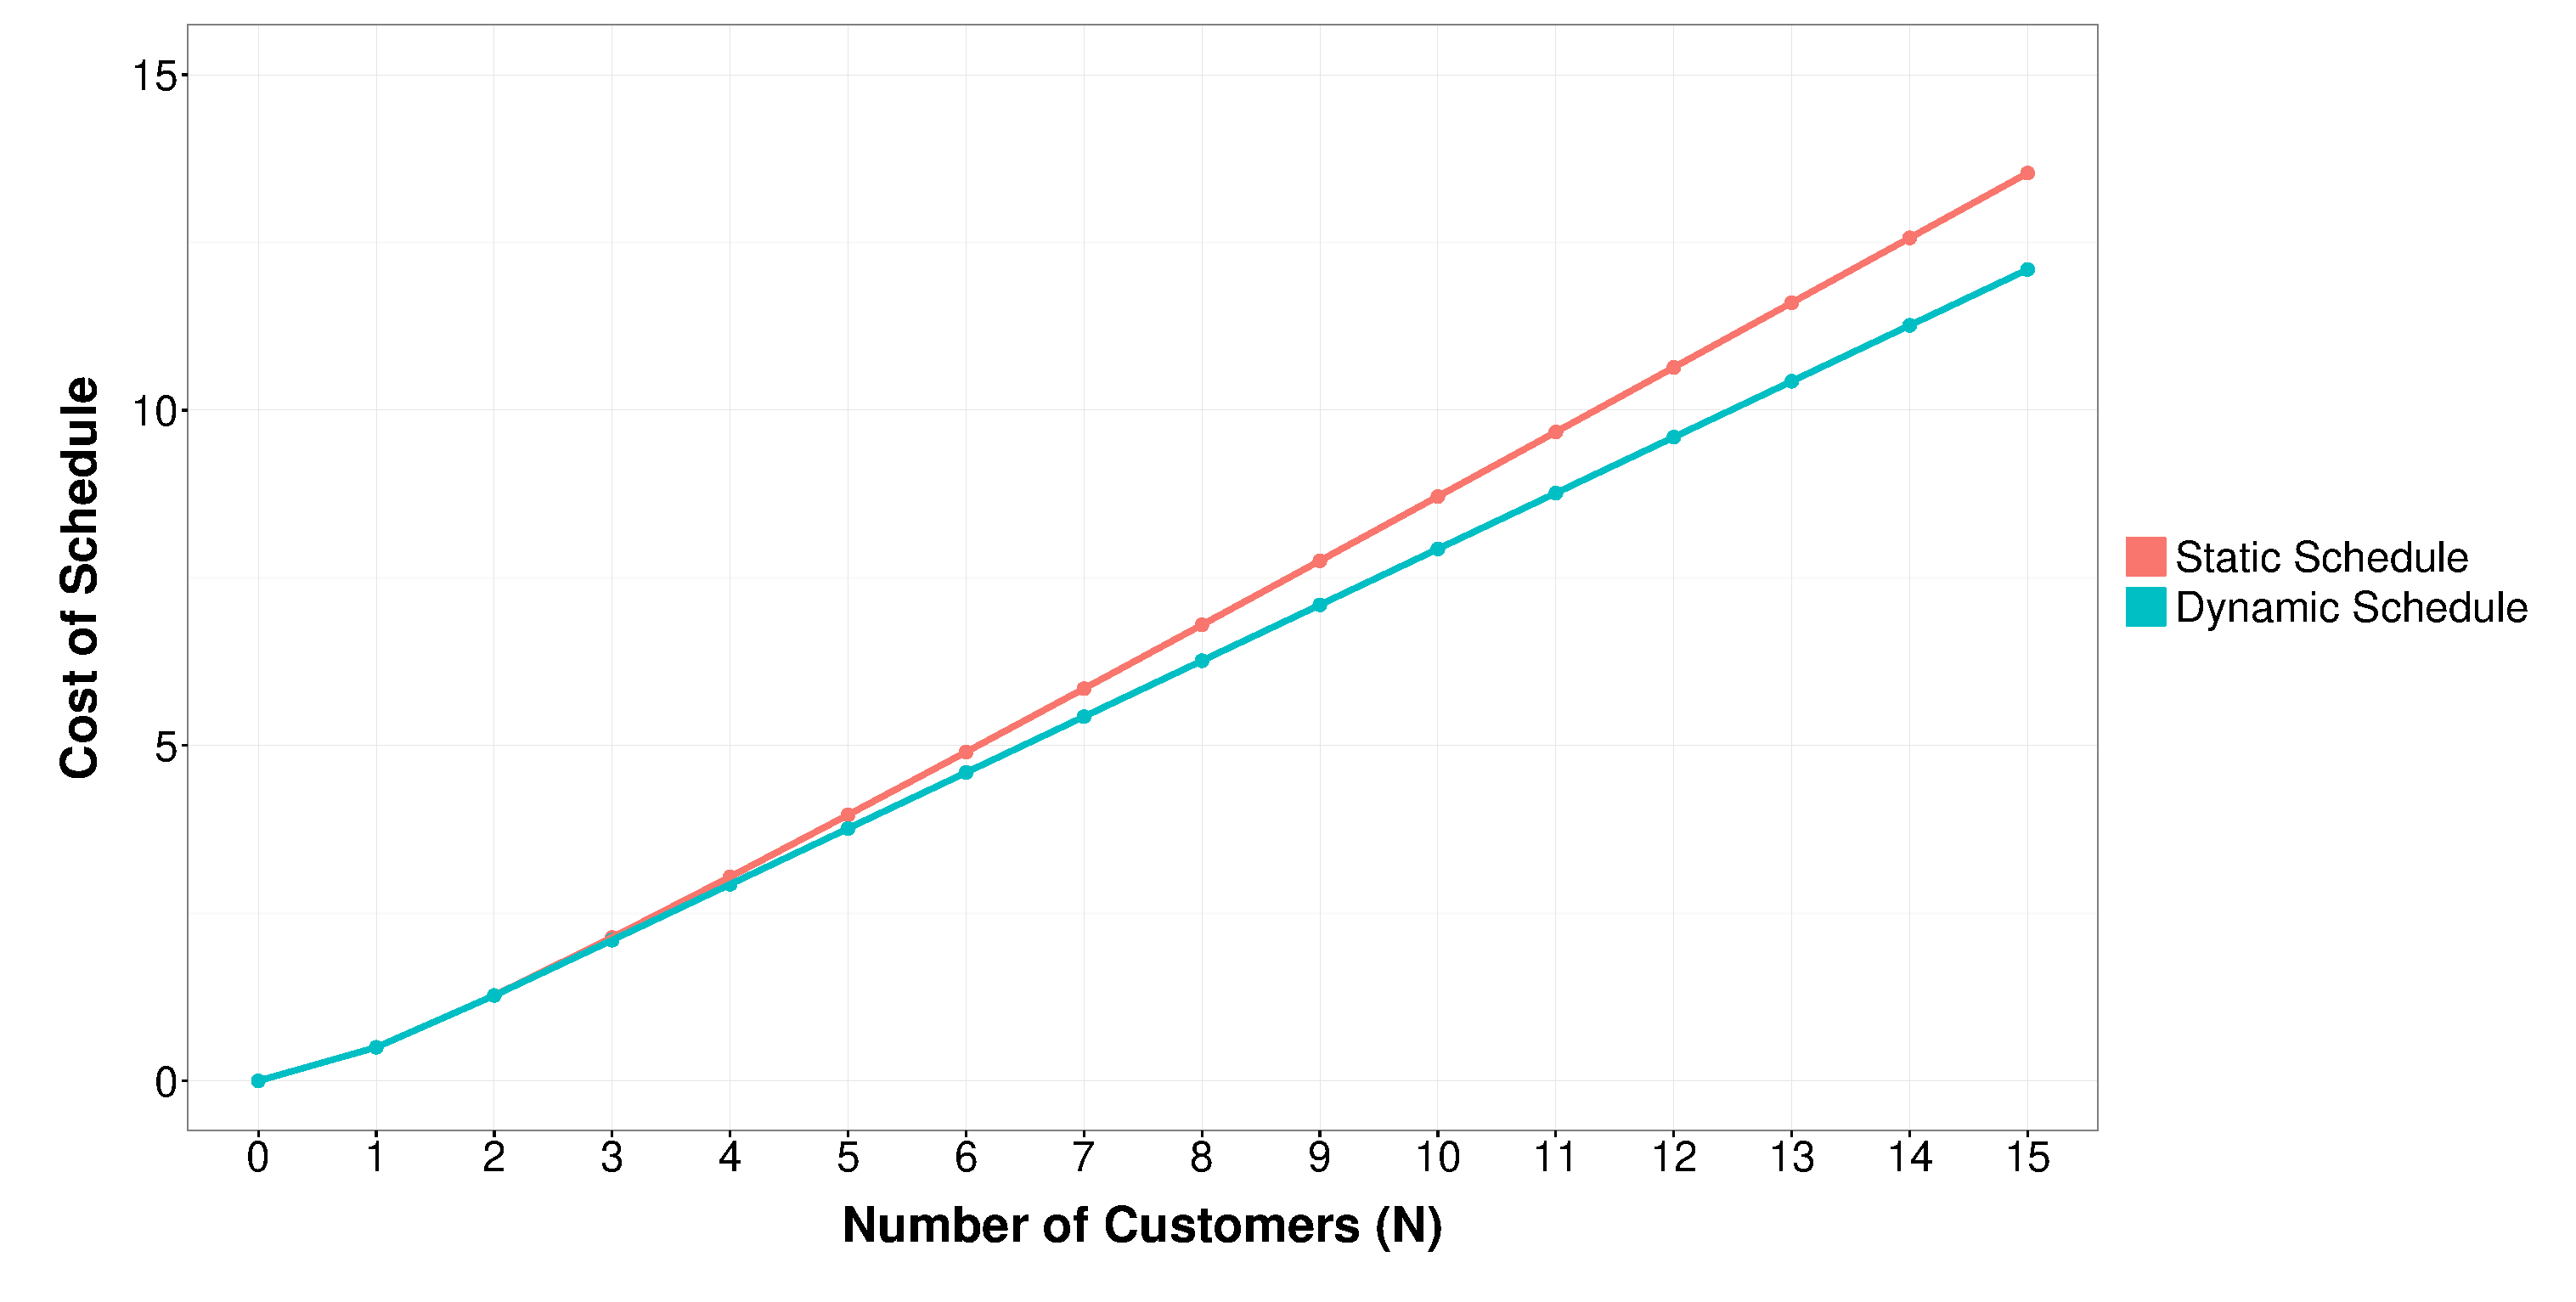
\includegraphics[width = 0.85\textwidth]{Comparison_Line_Cost_Num.eps}
	\caption{Plot of the expected cost of each schedule against the number of customers to be scheduled ($N$) for both the static and dynamic schedules where $N \in \{ 0, \ldots, 15 \}$, $\gamma = \frac{c_{S}}{c_{S} + c_{W}} = 0.5$ and $\mu = 1$.}
	\label{Graph_Cost_Comparison}
\end{figure}

As expected, the costs are identical for $N \in \{ 0, 1, 2 \}$. For all other $N$ values, the cost of the static schedule is greater than the cost of the dynamic schedule. The cost difference appears to be minimal for $N \geq 5$, but as $N$ increases the cost difference increases.

\section{Expected Percentage Cost Saving}
Define the expected percentage cost saving $\Delta C$ (i.e., the expected percentage difference between the cost of the static schedule and the dynamic schedule).
\begin{equation}
	\Delta C \coloneqq 100 \times \frac{\phi (\mathbf{x}_{N}^{*}) - C_{N}^{*} (0)}{\phi (\mathbf{x}_{N}^{*})}
\end{equation}

Figure~\ref{Graph_Cost_Saving} plots the percentage cost saving by using the dynamic schedule as opposed to the static schedule ($\Delta C$) against $\gamma$ for various values of the number of customers ($N$) to be scheduled. 
\begin{figure}[htb]
	\centering
	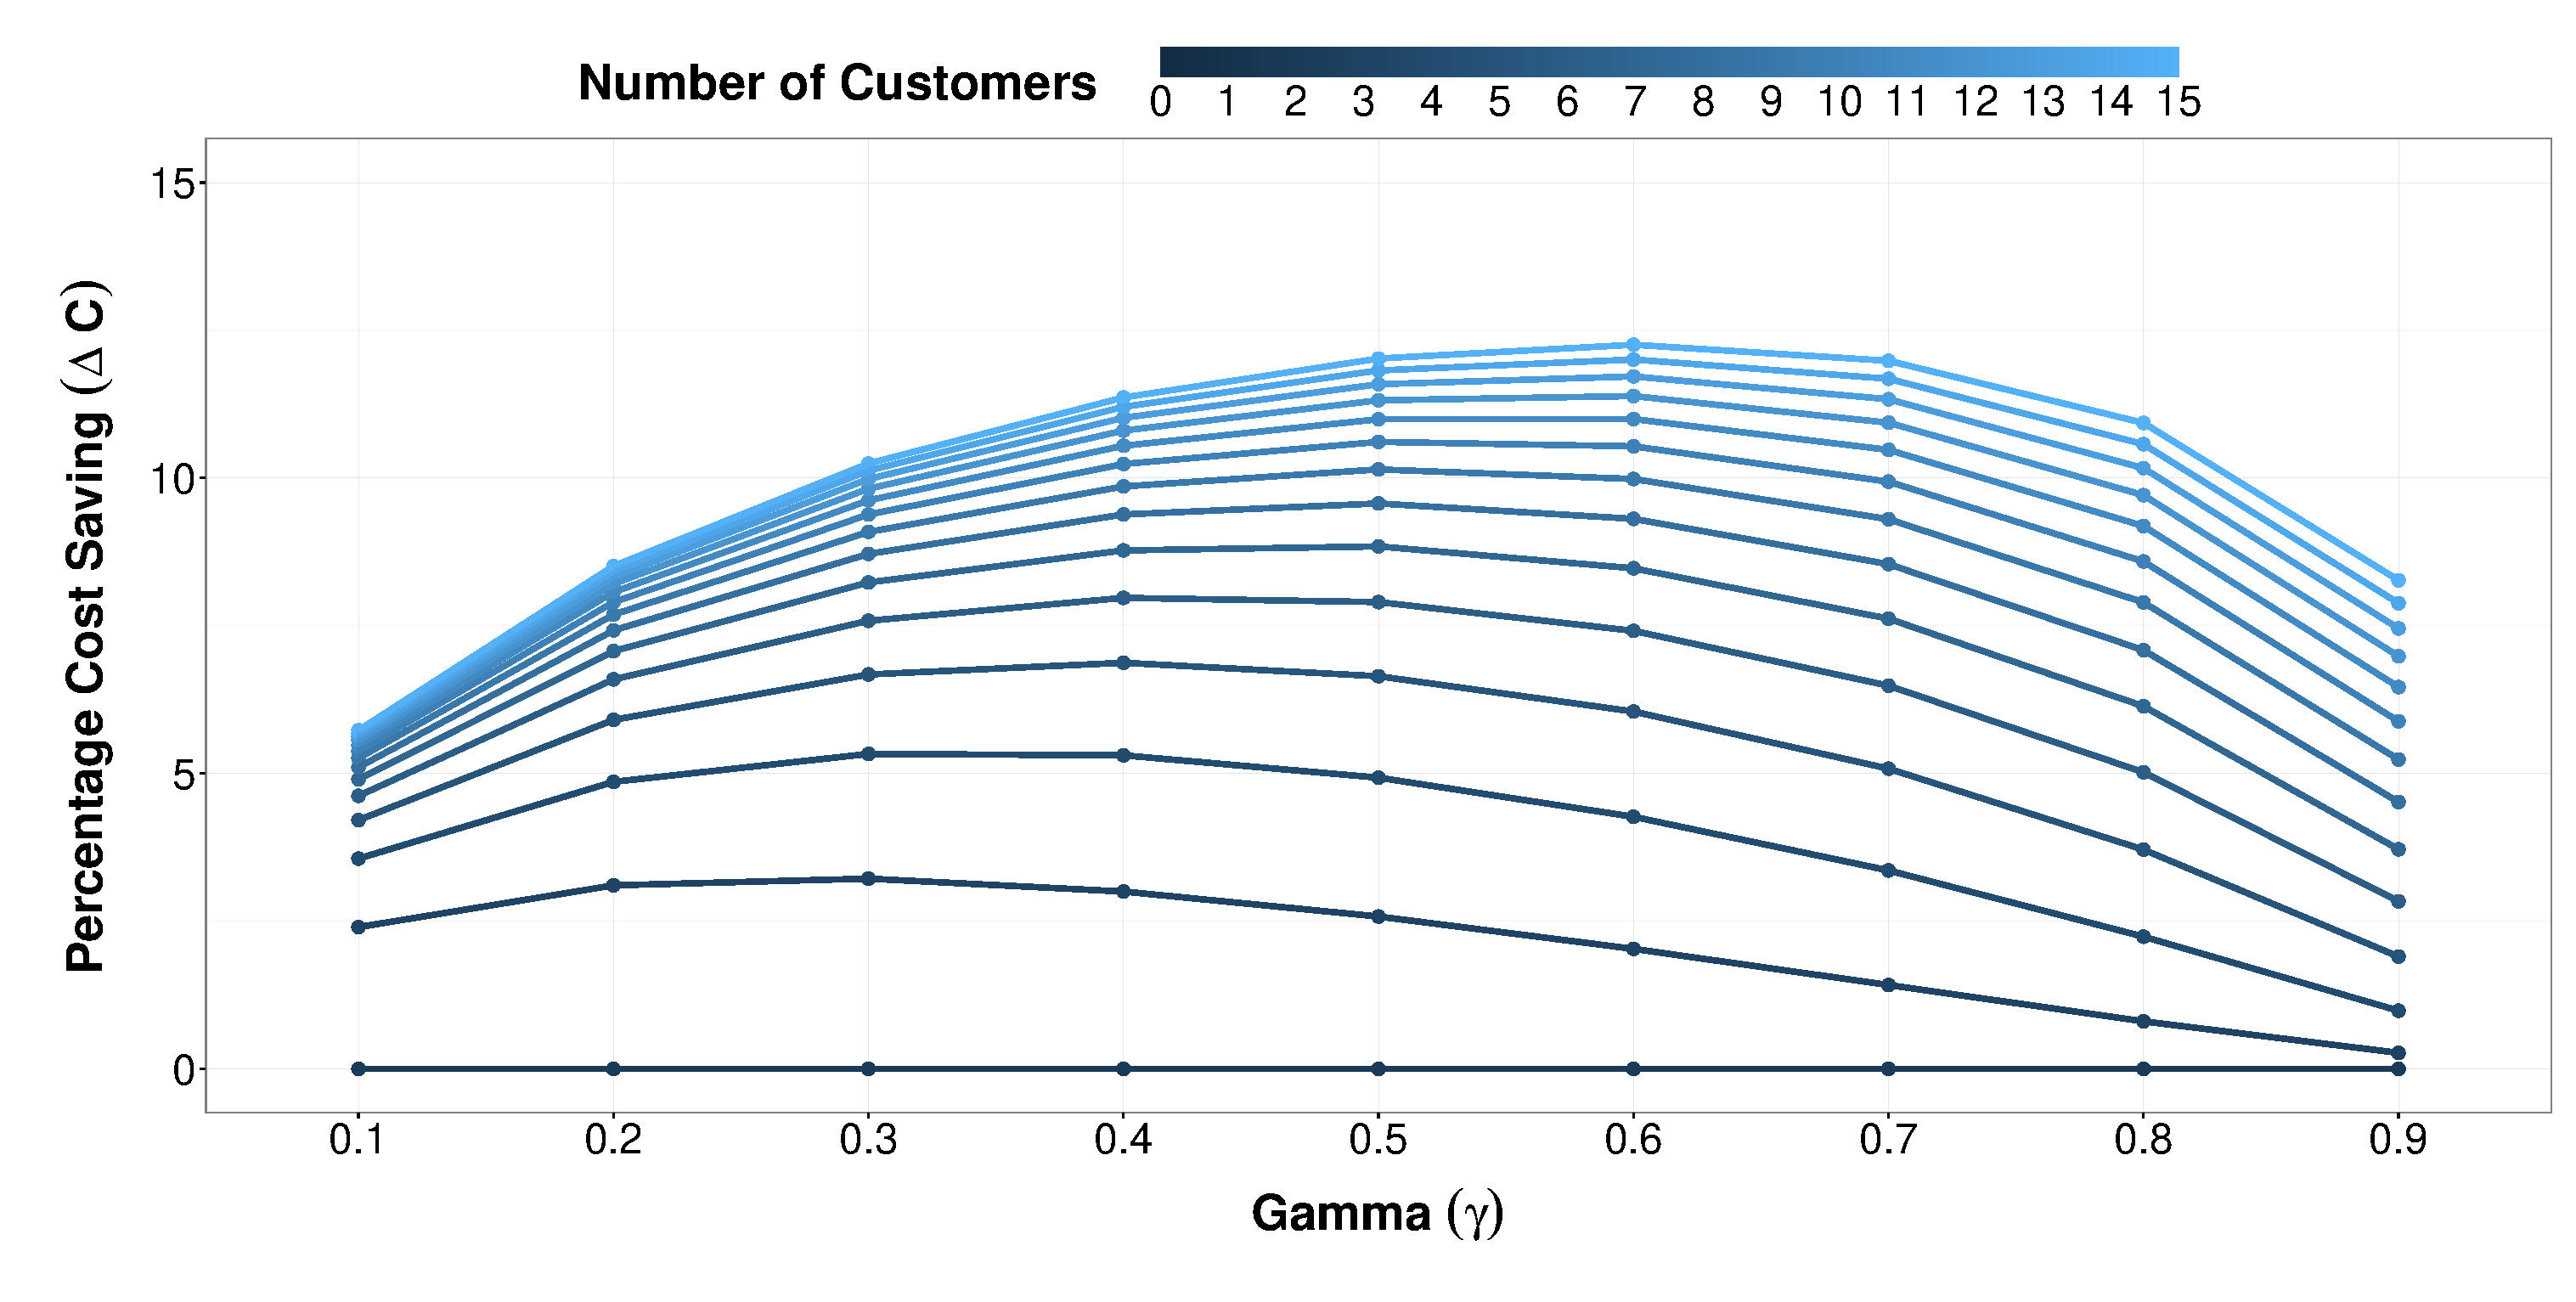
\includegraphics[width = 0.85\textwidth]{Cost_Saving_Line_Num.eps}
	\caption{Plot of the percentage cost saving ($\Delta C$) against $\gamma = \frac{c_{S}}{c_{S} + c_{W}}$ where $N = \{ 0, \ldots, 15 \}$ and $\mu = 1$.}
	\label{Graph_Cost_Saving}
\end{figure}

For $N \in \{ 0, 1, 2 \}$, $\Delta C = 0$ for all values of $\gamma$ as the schedules are identical. As $N$ increases with $\gamma$ held constant, $\Delta C$ increases as the dynamic schedule begins to outperform the static schedule. $\Delta C$ increases at a decreasing rate (i.e., the curves become closer together as $N$ increases). The maximal value of $\Delta C$ is $10.6 \%$. Even if $N$ were to increase further beyond $15$, it doesn't appear that the expected percentage cost saving would exceed $15 \%$.

For the extreme values of $\gamma$ (i.e., $\gamma = 0.1$ and $\gamma = 0.9$), $\Delta C$ is at a minimum for each value of $N$. An extreme value of $\gamma$ indicates that the either the customer waiting cost or the server availability cost is significantly priorities (i.e., $c_{W} \gg c_{S}$ or $c_{S} \gg c_{W}$). If one of the costs is heavily prioritised, there is little difference between the static and dynamic schedules, thus $\Delta C$ is small.

For each value of $N \geq 3$, the peak value of $\Delta C$ occurs at a middle value of $\gamma$. As $N$ increases, the peak occurs at a larger value of $\gamma$. For $N = 3$ the peak occurs at $\gamma = 0.3$, whereas for $N = 15$ the peak occurs at $\gamma = 0.7$.

The difference between the dynamic and static schedule is most significant for middle values of $\gamma$ (e.g., $\gamma \in [0.4, 0.7]$). For $\gamma = 0.1$, it doesn't appear that the expected percentage cost saving would exceed $5 \%$ indicating very little difference between the schedules.

\chapter{Simulation Studies}
\label{chap:Simulation}
The previous chapter compared the static and dynamic schedules in terms of the expected cost of each schedule. We found for $15$ customers, the dynamic schedule is about $5 - 10 \%$ better than the static schedule depending on the value of $\gamma$. However, this does not provide any information about the other properties of each schedule. For example, one of the scheduled could have a greater variability in customer waiting times.

To understand each schedule more fully, we'll use a simulation study. We simulated a million runs and measured the performance of both the static and dynamic schedules on each run. Each run involved simulating the service times of the $15$ customers assuming $\mu = 1$. All the simulations were completed assuming $\gamma = 0.5$.

\section{Schedule Cost}
The mean costs of the static and dynamic schedule were $15.05$ and $13.55$ respectively. As expected, these mean costs match closely the expected costs of the schedules. Figure~\ref{fig:Two_Cost} plots the histograms of the costs of the static and dynamic schedules for each run of the simulation.
\begin{figure}[htb]
	\centering
	\begin{subfigure}[t]{0.45\textwidth}
		\centering
		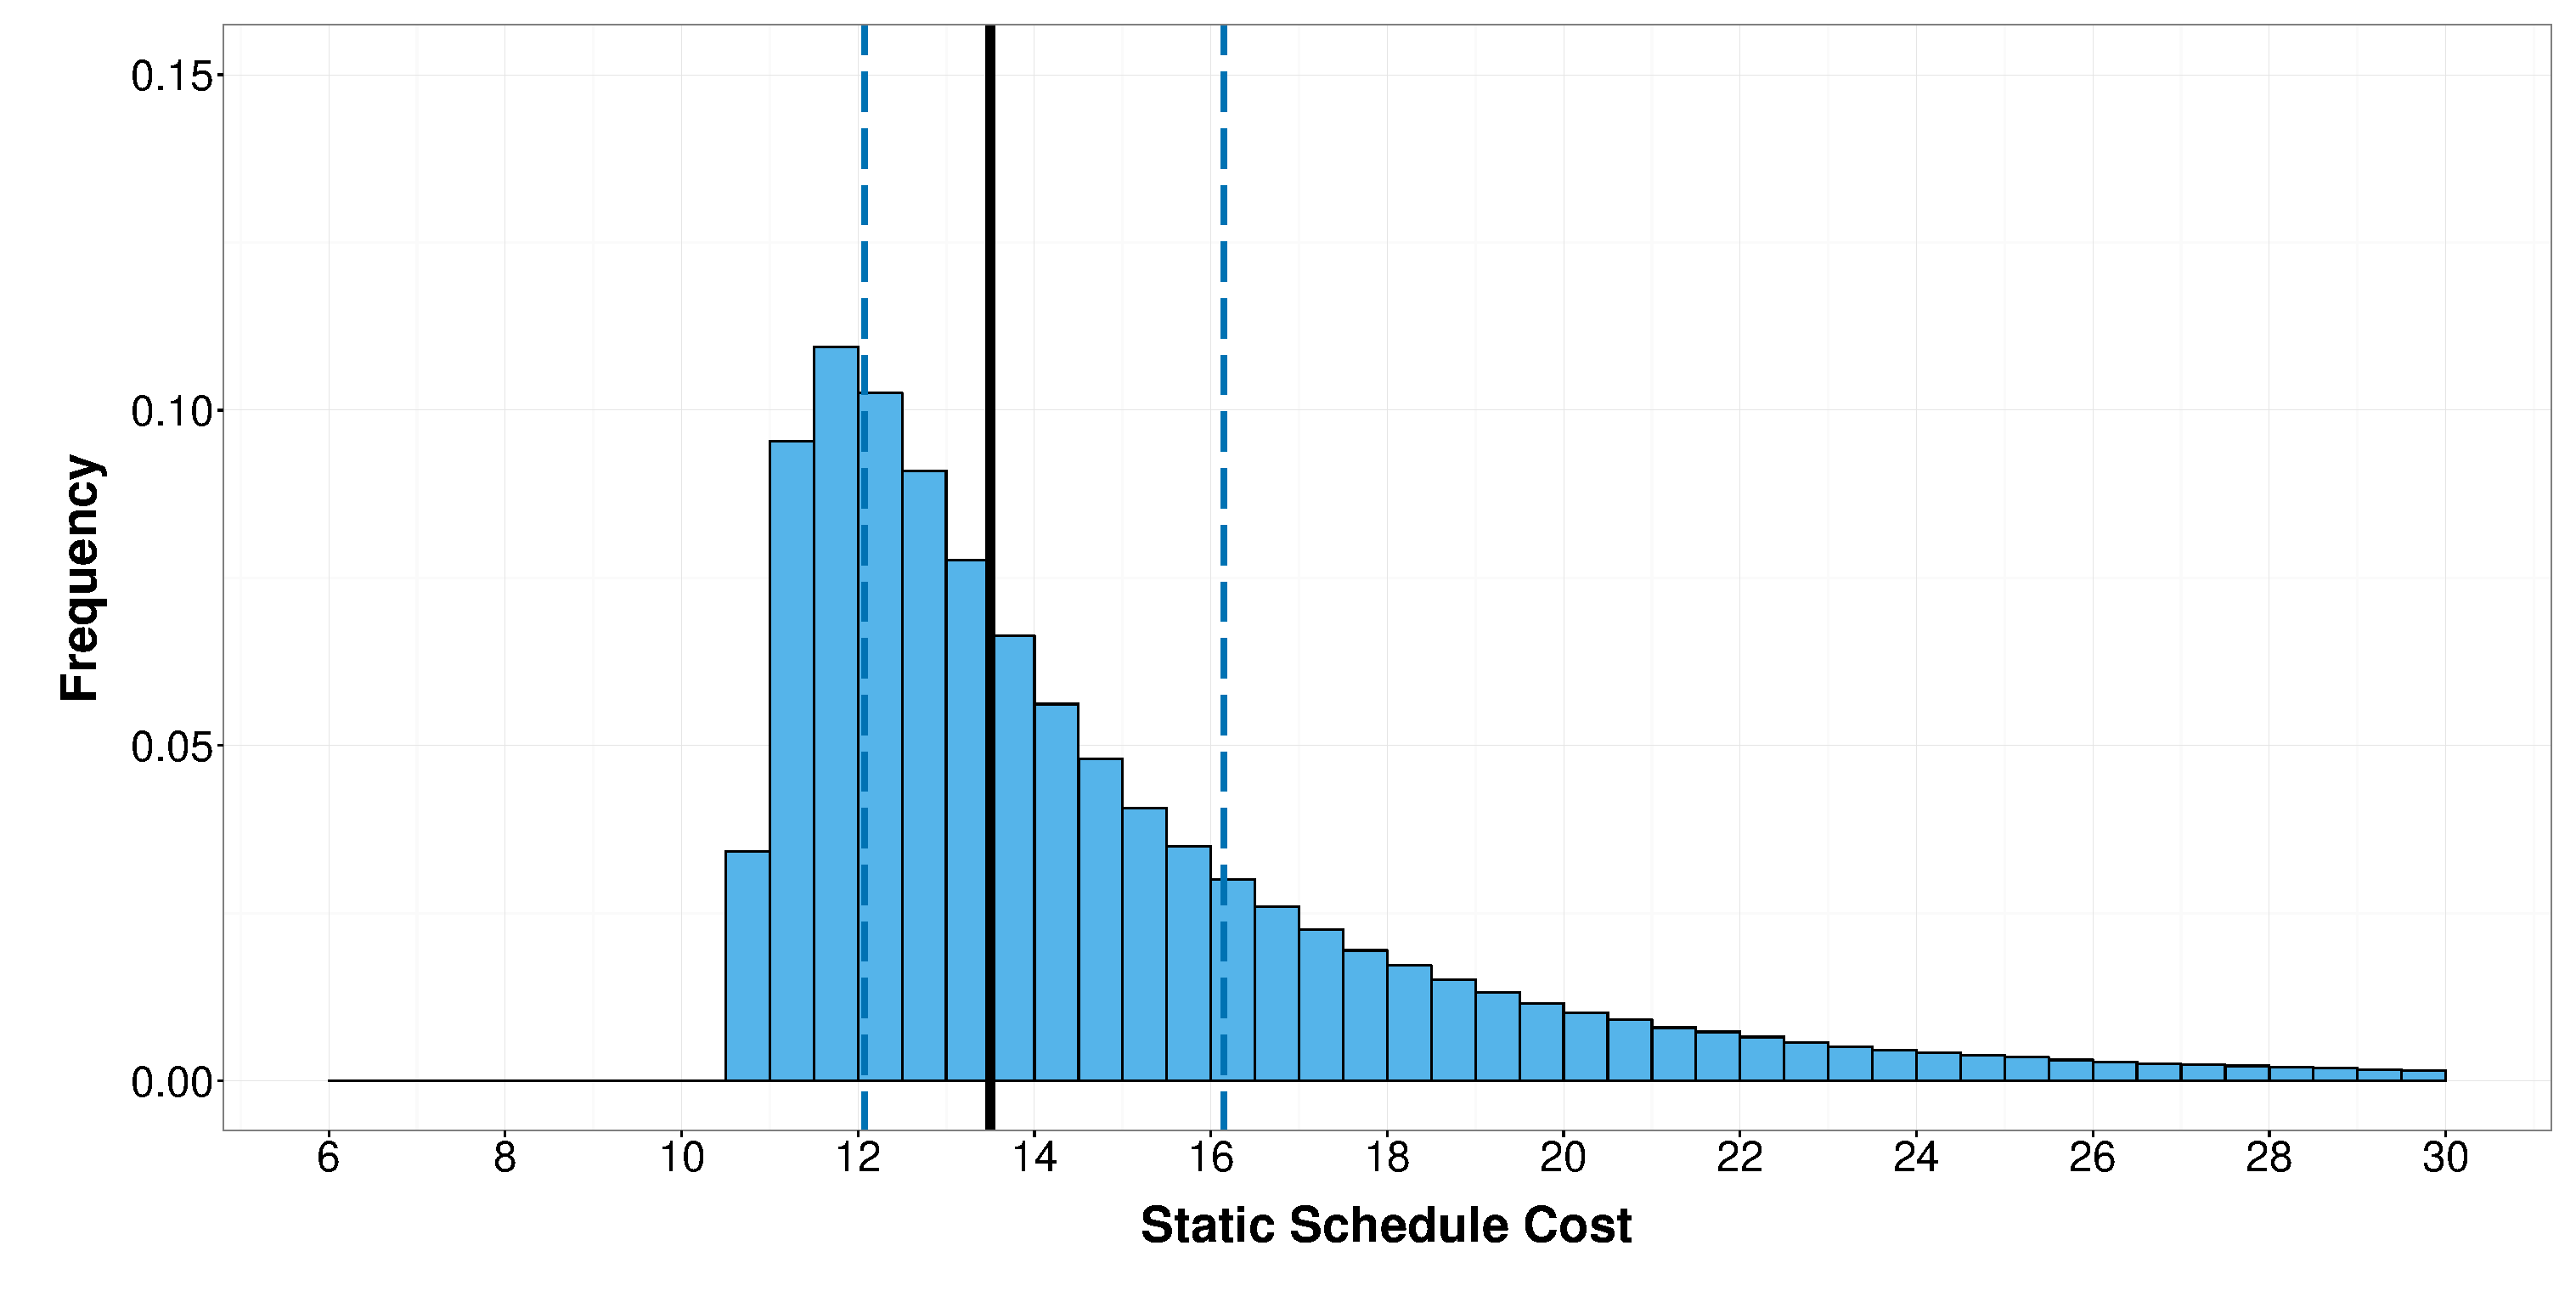
\includegraphics[width=\textwidth]{Cost_Hist_Static.eps}
		\caption{}
	\end{subfigure}
	\begin{subfigure}[t]{0.45\textwidth}
		\centering
		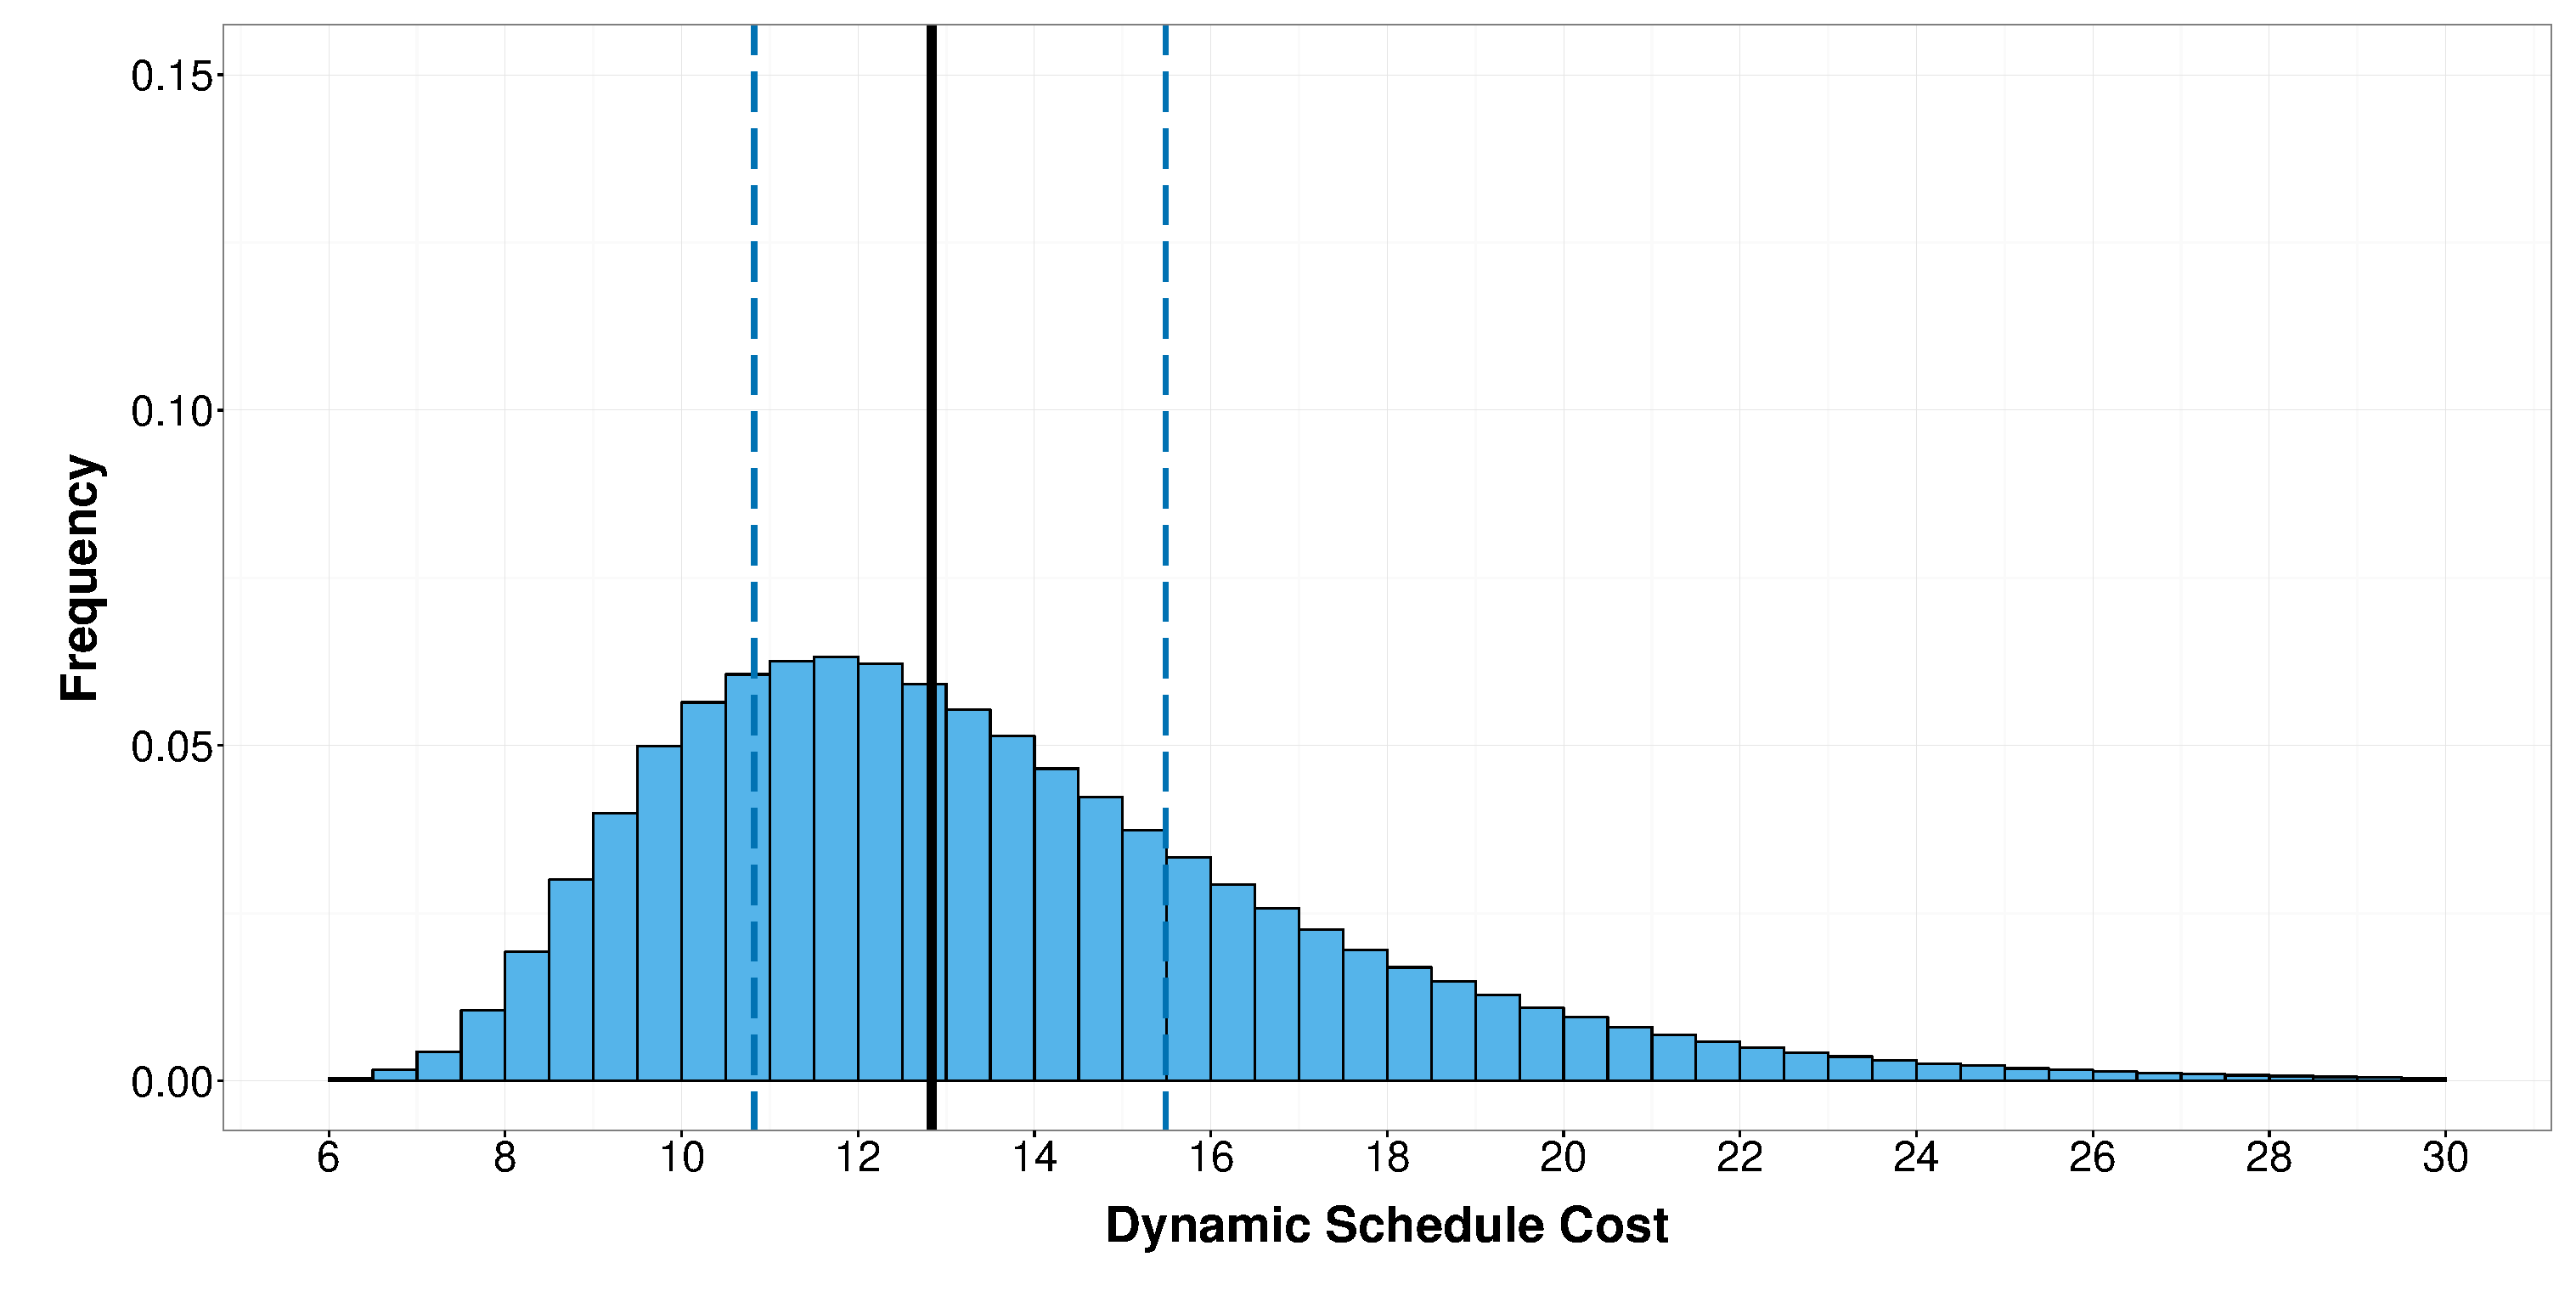
\includegraphics[width=\textwidth]{Cost_Hist_Dynamic.eps}
		\caption{}
	\end{subfigure}
	\caption{Histogram plot of the costs of the static (a) and dynamic (b) schedules for each simulation run where $\mu = 1$ and $\gamma = \frac{c_{S}}{c_{S} + c_{W}} = 0.5$. The black vertical line indicates the median and the blue dashes lines indicate the upper and lower quartiles.}
	\label{fig:Two_Cost}
\end{figure}

The distribution of the cost of the static schedule is right skewed. The peak of the distribution occurs at around 12, but the median is $13.5$. In contrast, the distribution of the dynamic schedule is more symmetric with the peak ocurring much closer to the median of $12.8$. The dynamic schedule is more flexible and thus less prone to runs with high cost.

Figure~\ref{fig:Diff_Cost} plots the histogram of the difference in costs between the two schedules. This is a plot of the cost of the static schedule minus the cost of the dynamic schedule for the same run.
\begin{figure}[htb]
	\centering
	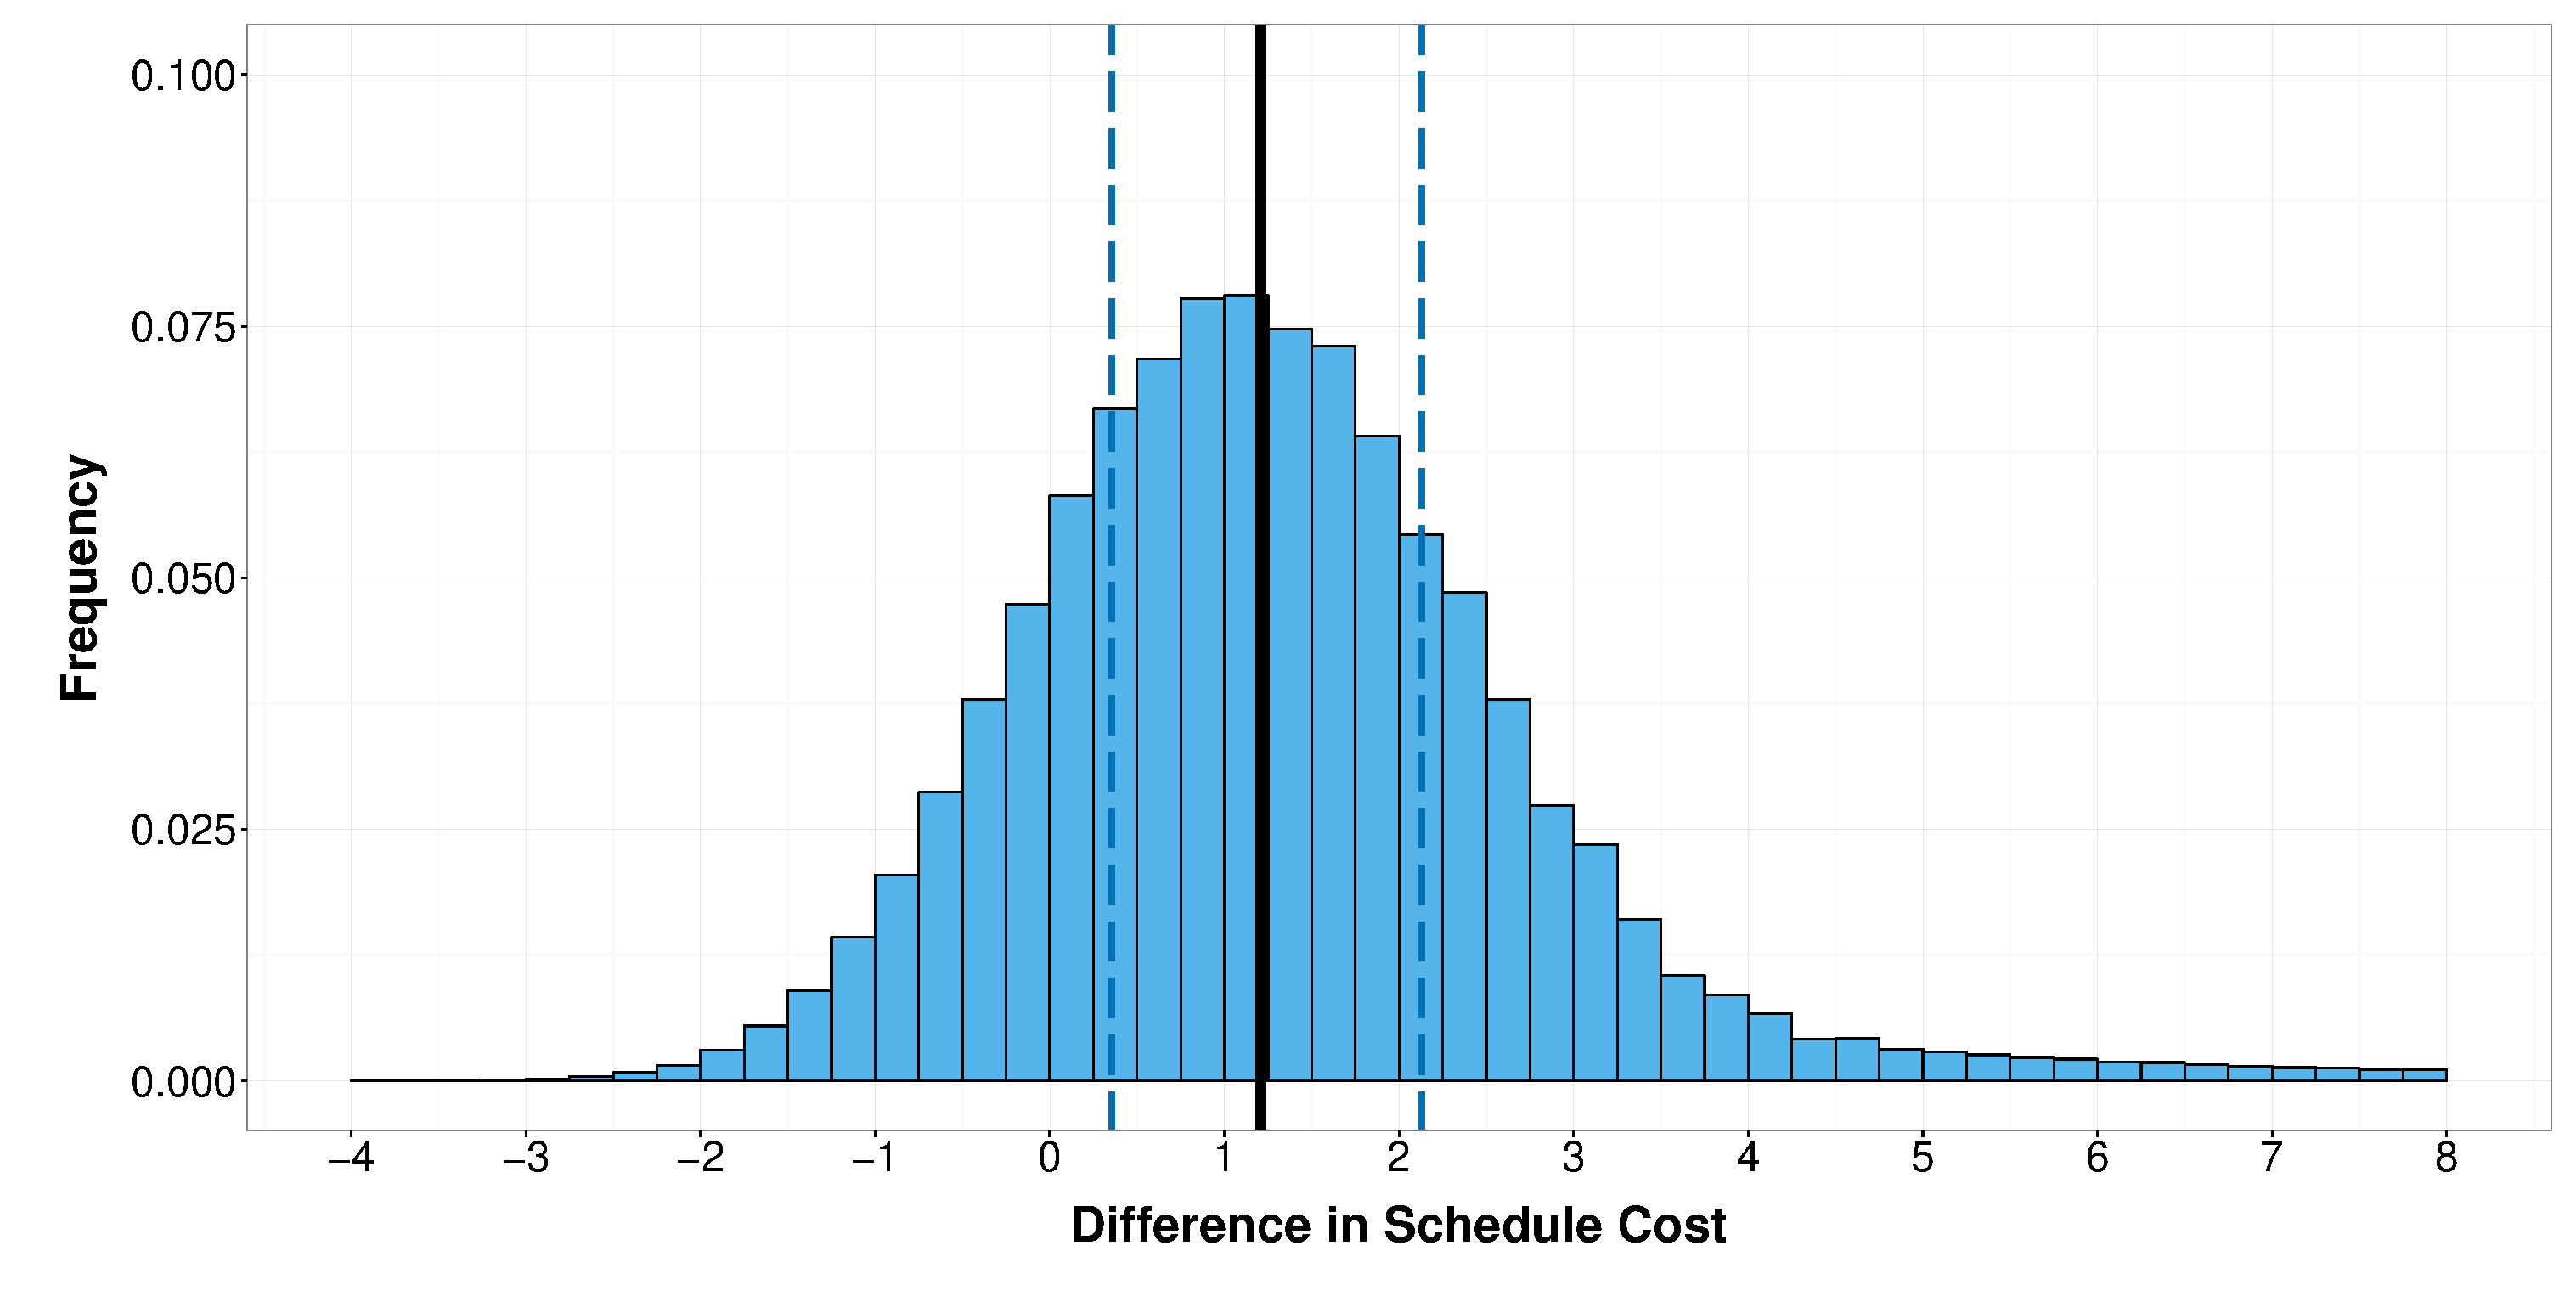
\includegraphics[width = 0.85\textwidth]{Cost_Hist_Diff.eps}
	\caption{Histogram plot of the cost of the static schedule minus the cost of the dynamic schedule for each simulation run where $\mu = 1$ and $\gamma = \frac{c_{S}}{c_{S} + c_{W}} = 0.5$. The black vertical line indicates the median and the blue dashes lines indicate the upper and lower quartiles.}
	\label{fig:Diff_Cost}
\end{figure}

While the expected cost of the static schedule is greater than the expected cost of the dynamic schedule, the static schedule outperforms the dynamic schedule for a proportion of the simulation runs. This is indicated by a negative cost difference in the plotted histogram. The $25$-th percentile of the difference in cost is $0.35$. For more than $75 \%$ of runs, the static schedule has a larger cost than the dynamic schedule. The $75$-th percentile is $2.13$ (i.e., more than twice the mean service time). For a large proportion of the runs, the dynamic schedule significantly outperforms the static schedule.

\section{Customer Arrival Times}
We have now observed that the dynamic schedule performs better than the static schedule both in expectation and for the majority of the simulation runs. The next step is to attempt to understand how the dynamic schedule is able to outperform the static schedule. Figure~\ref{fig:Avg_Arrival} plots the average arrival time for each of the $15$ customers for each schedule.
\begin{figure}[htb]
	\centering
	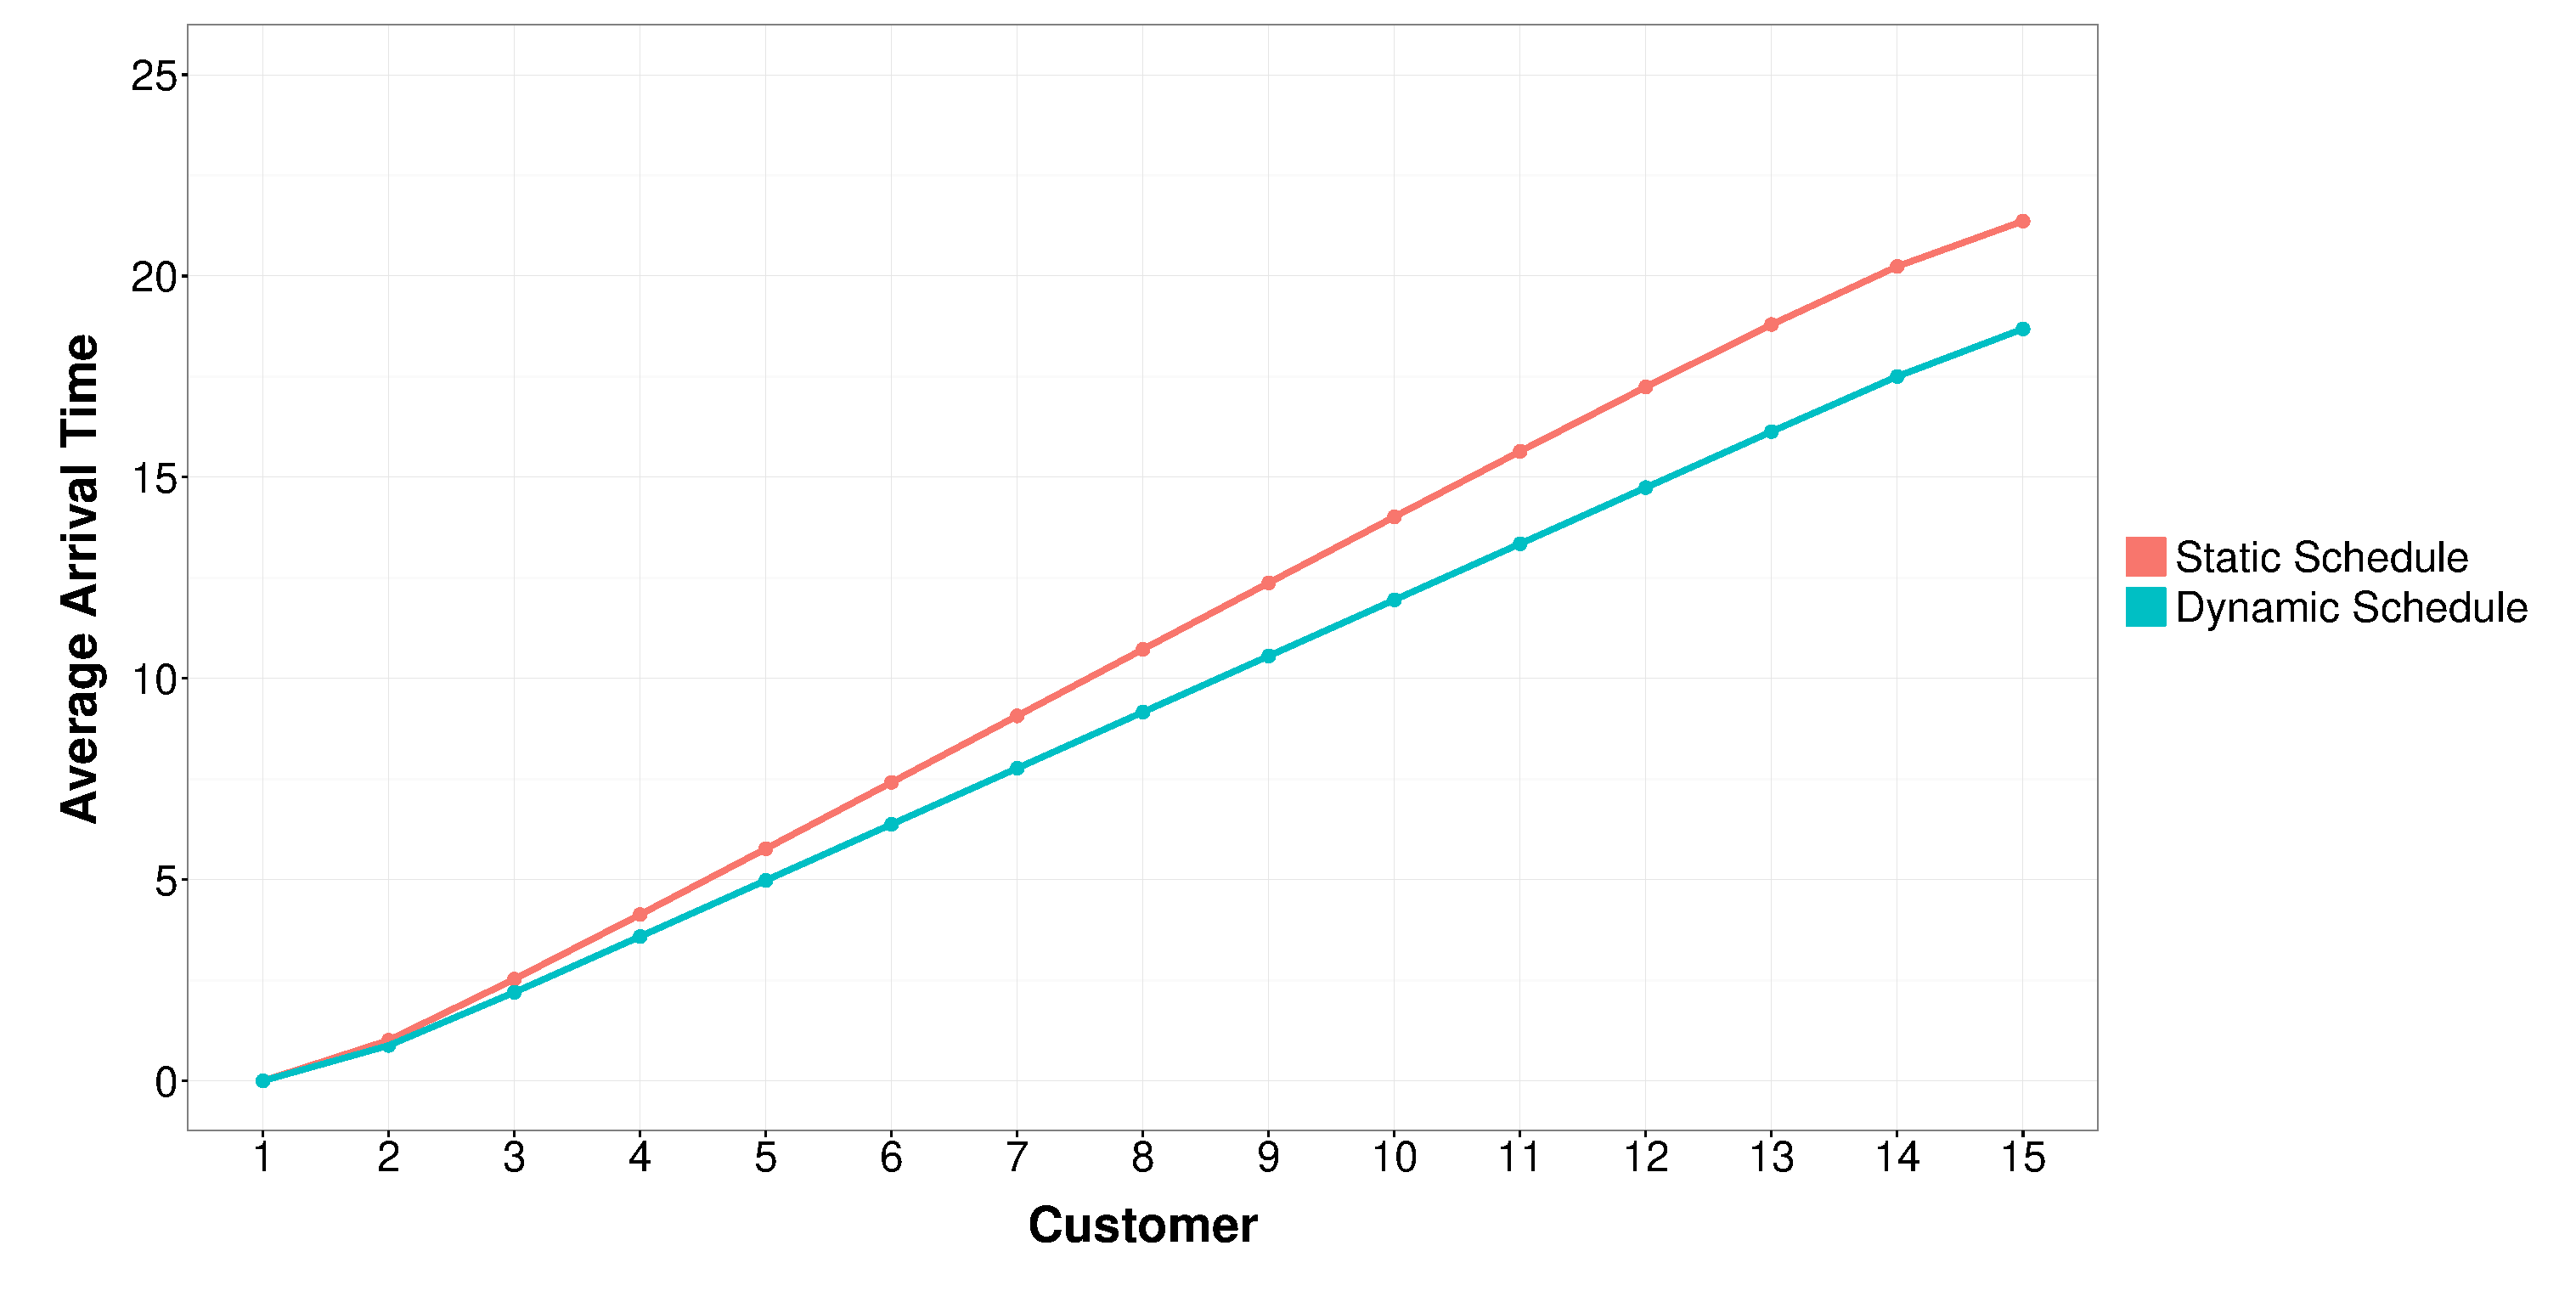
\includegraphics[width = 0.85\textwidth]{AT_Line.eps}
	\caption{Plot of the average arrival time for each of the $15$ customers for each schedule where $\mu = 1$ and $\gamma = \frac{c_{S}}{c_{S} + c_{W}} = 0.5$.}
	\label{fig:Avg_Arrival}
\end{figure}

The static schedule has fixed arrival times, whereas the arrival times are chosen progressively for the dynamic schedule. For all $15$ customers, the mean arrival time for the dynamic schedule is never earlier than the arrival time of the static schedule. The mean arrival times appear to be very similar for the first four or five customers. However, the later customers in the dynamic schedule appear to arrive significantly earler than the corresponding customers in the static schedule.

\section{Customer Waiting Times}
We would expect that the earlier arrival of the customers in the dynamic schedule would lead to those customers waiting longer. This hypothesis is examined by plotting the histogram of the difference in average customer waiting time between the two schedule in Figure~\ref{fig:Diff_Wait}. As before, this is a plot of the average waiting time of the static schedule minus the average waiting time of the dynamic schedule.
\begin{figure}[htb]
	\centering
	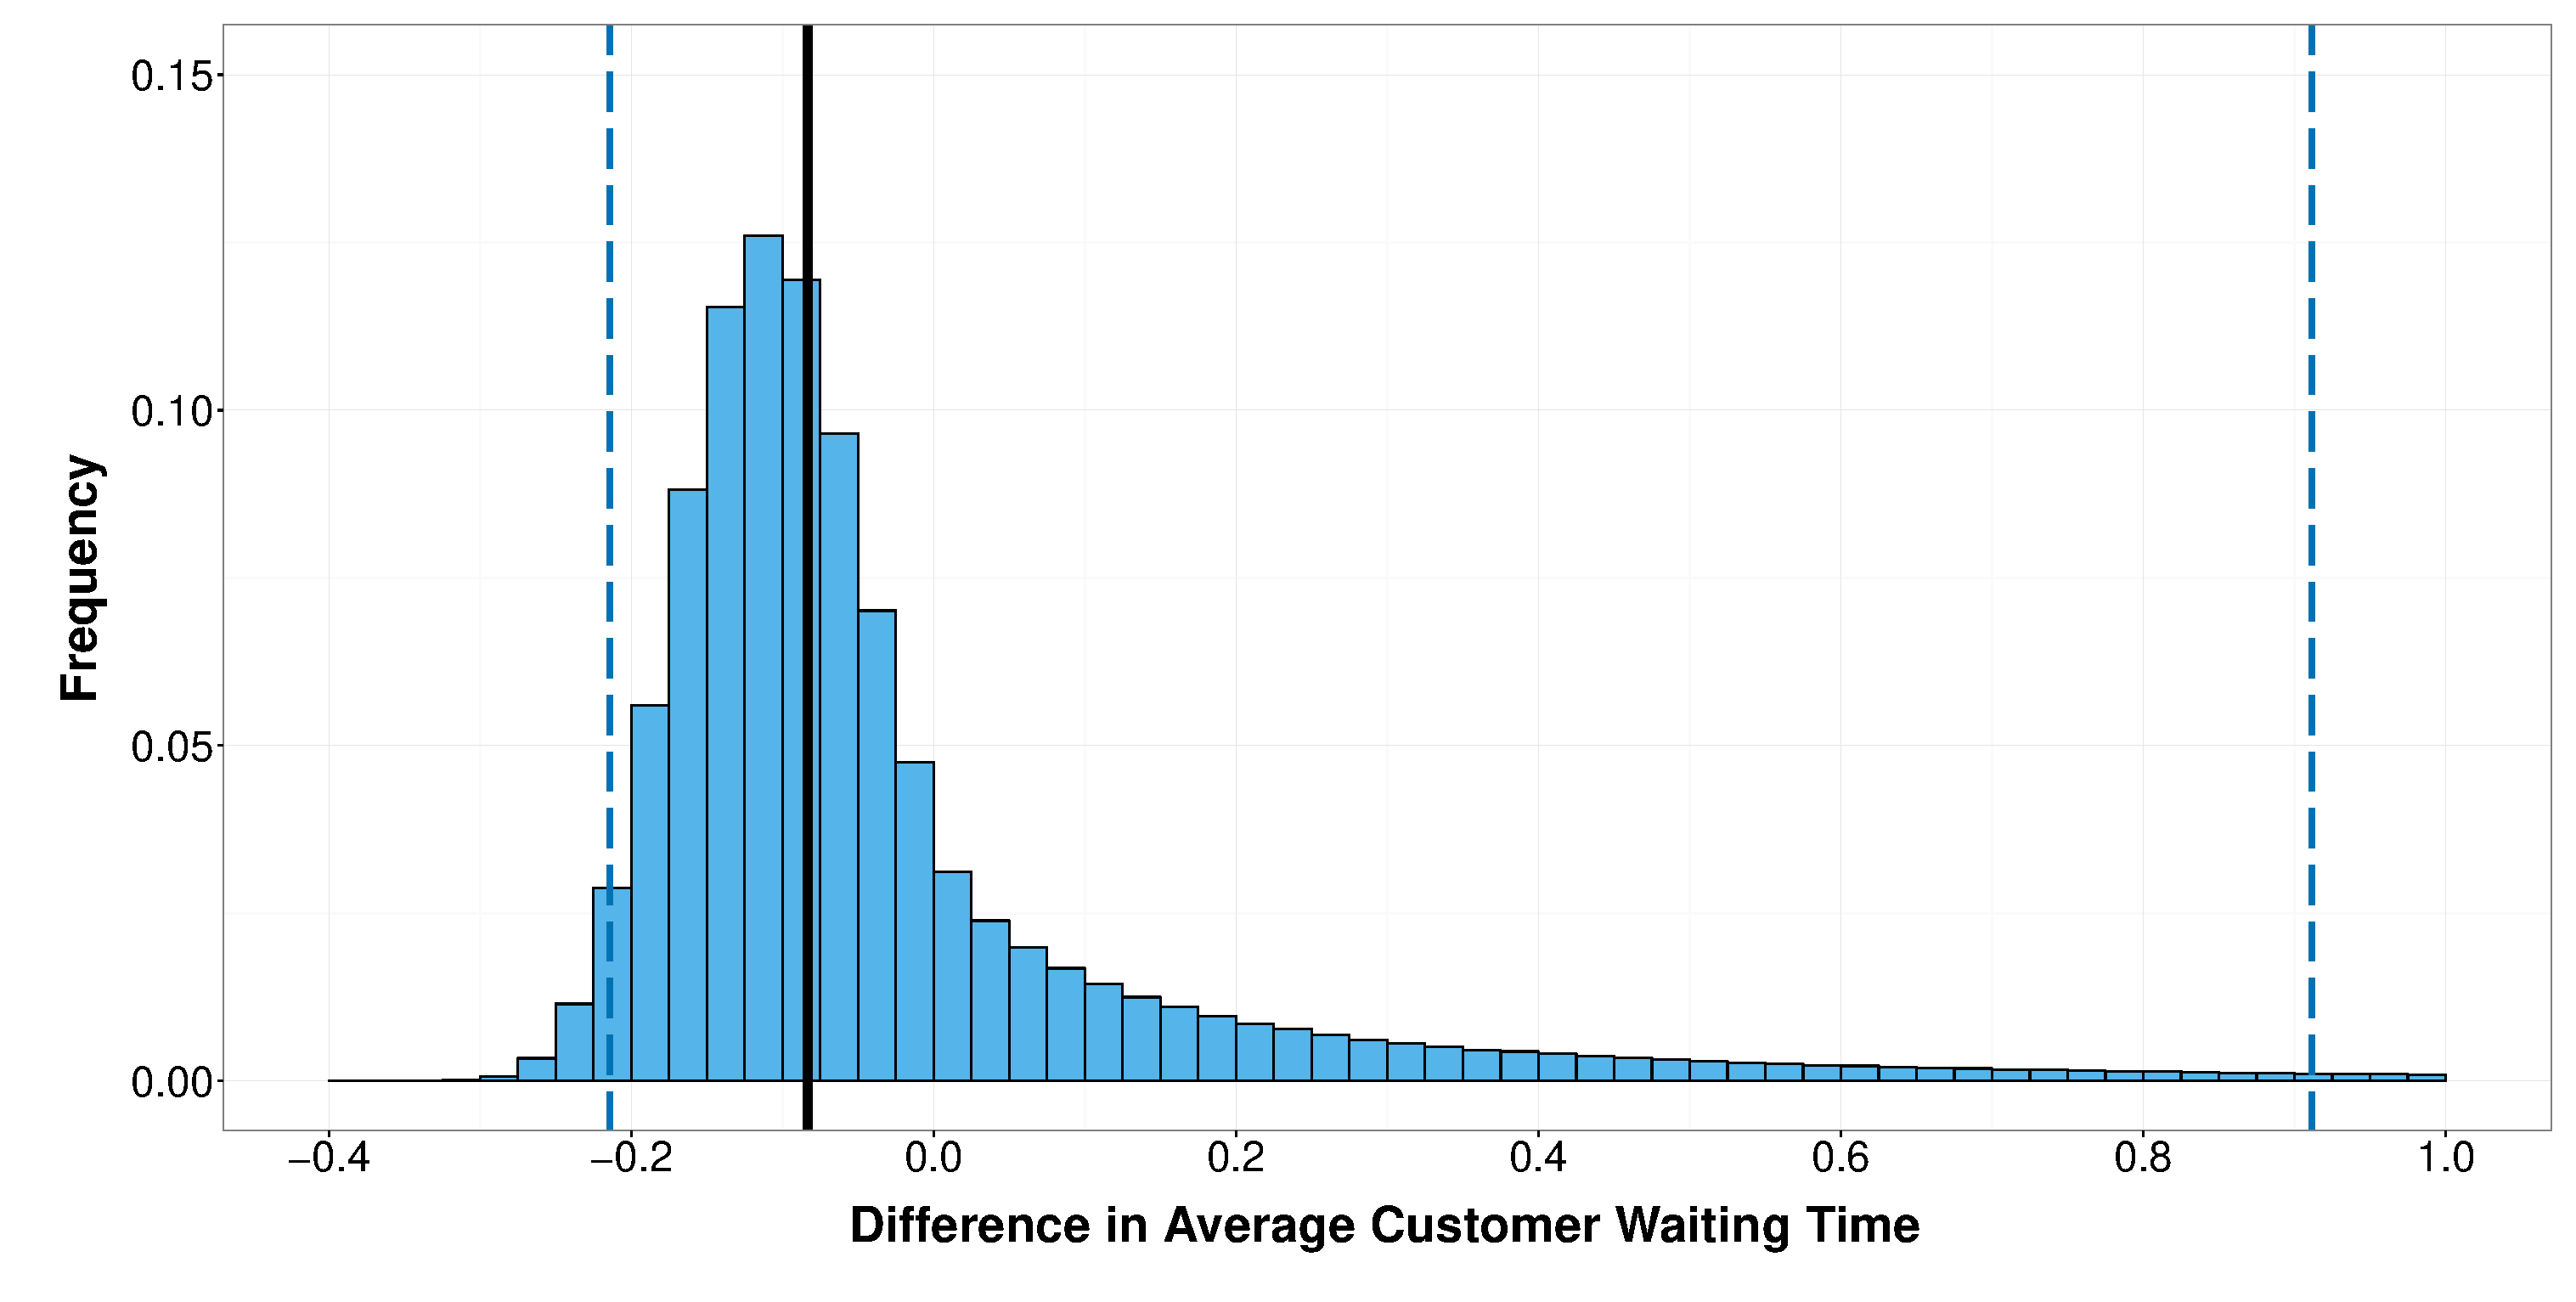
\includegraphics[width = 0.85\textwidth]{WT_Hist_Diff.eps}
	\caption{Histogram plot of the average waiting time for the static schedule minus the average waiting time for the dynamic schedule where $\mu = 1$ and $\gamma = \frac{c_{S}}{c_{S} + c_{W}} = 0.5$. The black vertical line indicates the median and the blue dashes lines indicate the upper and lower quartiles.}
	\label{fig:Diff_Wait}
\end{figure}

The $75$-th percentile of the difference in average waiting time is $0$. As expected, for the majority of the runs, the customers in the static schedule have a shorter average waiting time than the customers in the dynamic schedule.

However, the minimum difference in average waiting time is only $-0.33$, whereas the maximum is $8.57$. It appears that when the dynamic schedule has a shorter waiting time than the static schedule, it tends to have a significantly shorter waiting time. The dynamic schedule is less prone to extremely long waiting times for the customers. This is expected behaviour as the dynamic schedule is able to react to customers having longer than expected service times and reschedule the later customers.

Another important consideration is the treatment of all the customers individually. Figure~\ref{fig:Avg_Wait_Position} plots the average waiting time of each customer individually.
\begin{figure}[htb]
	\centering
	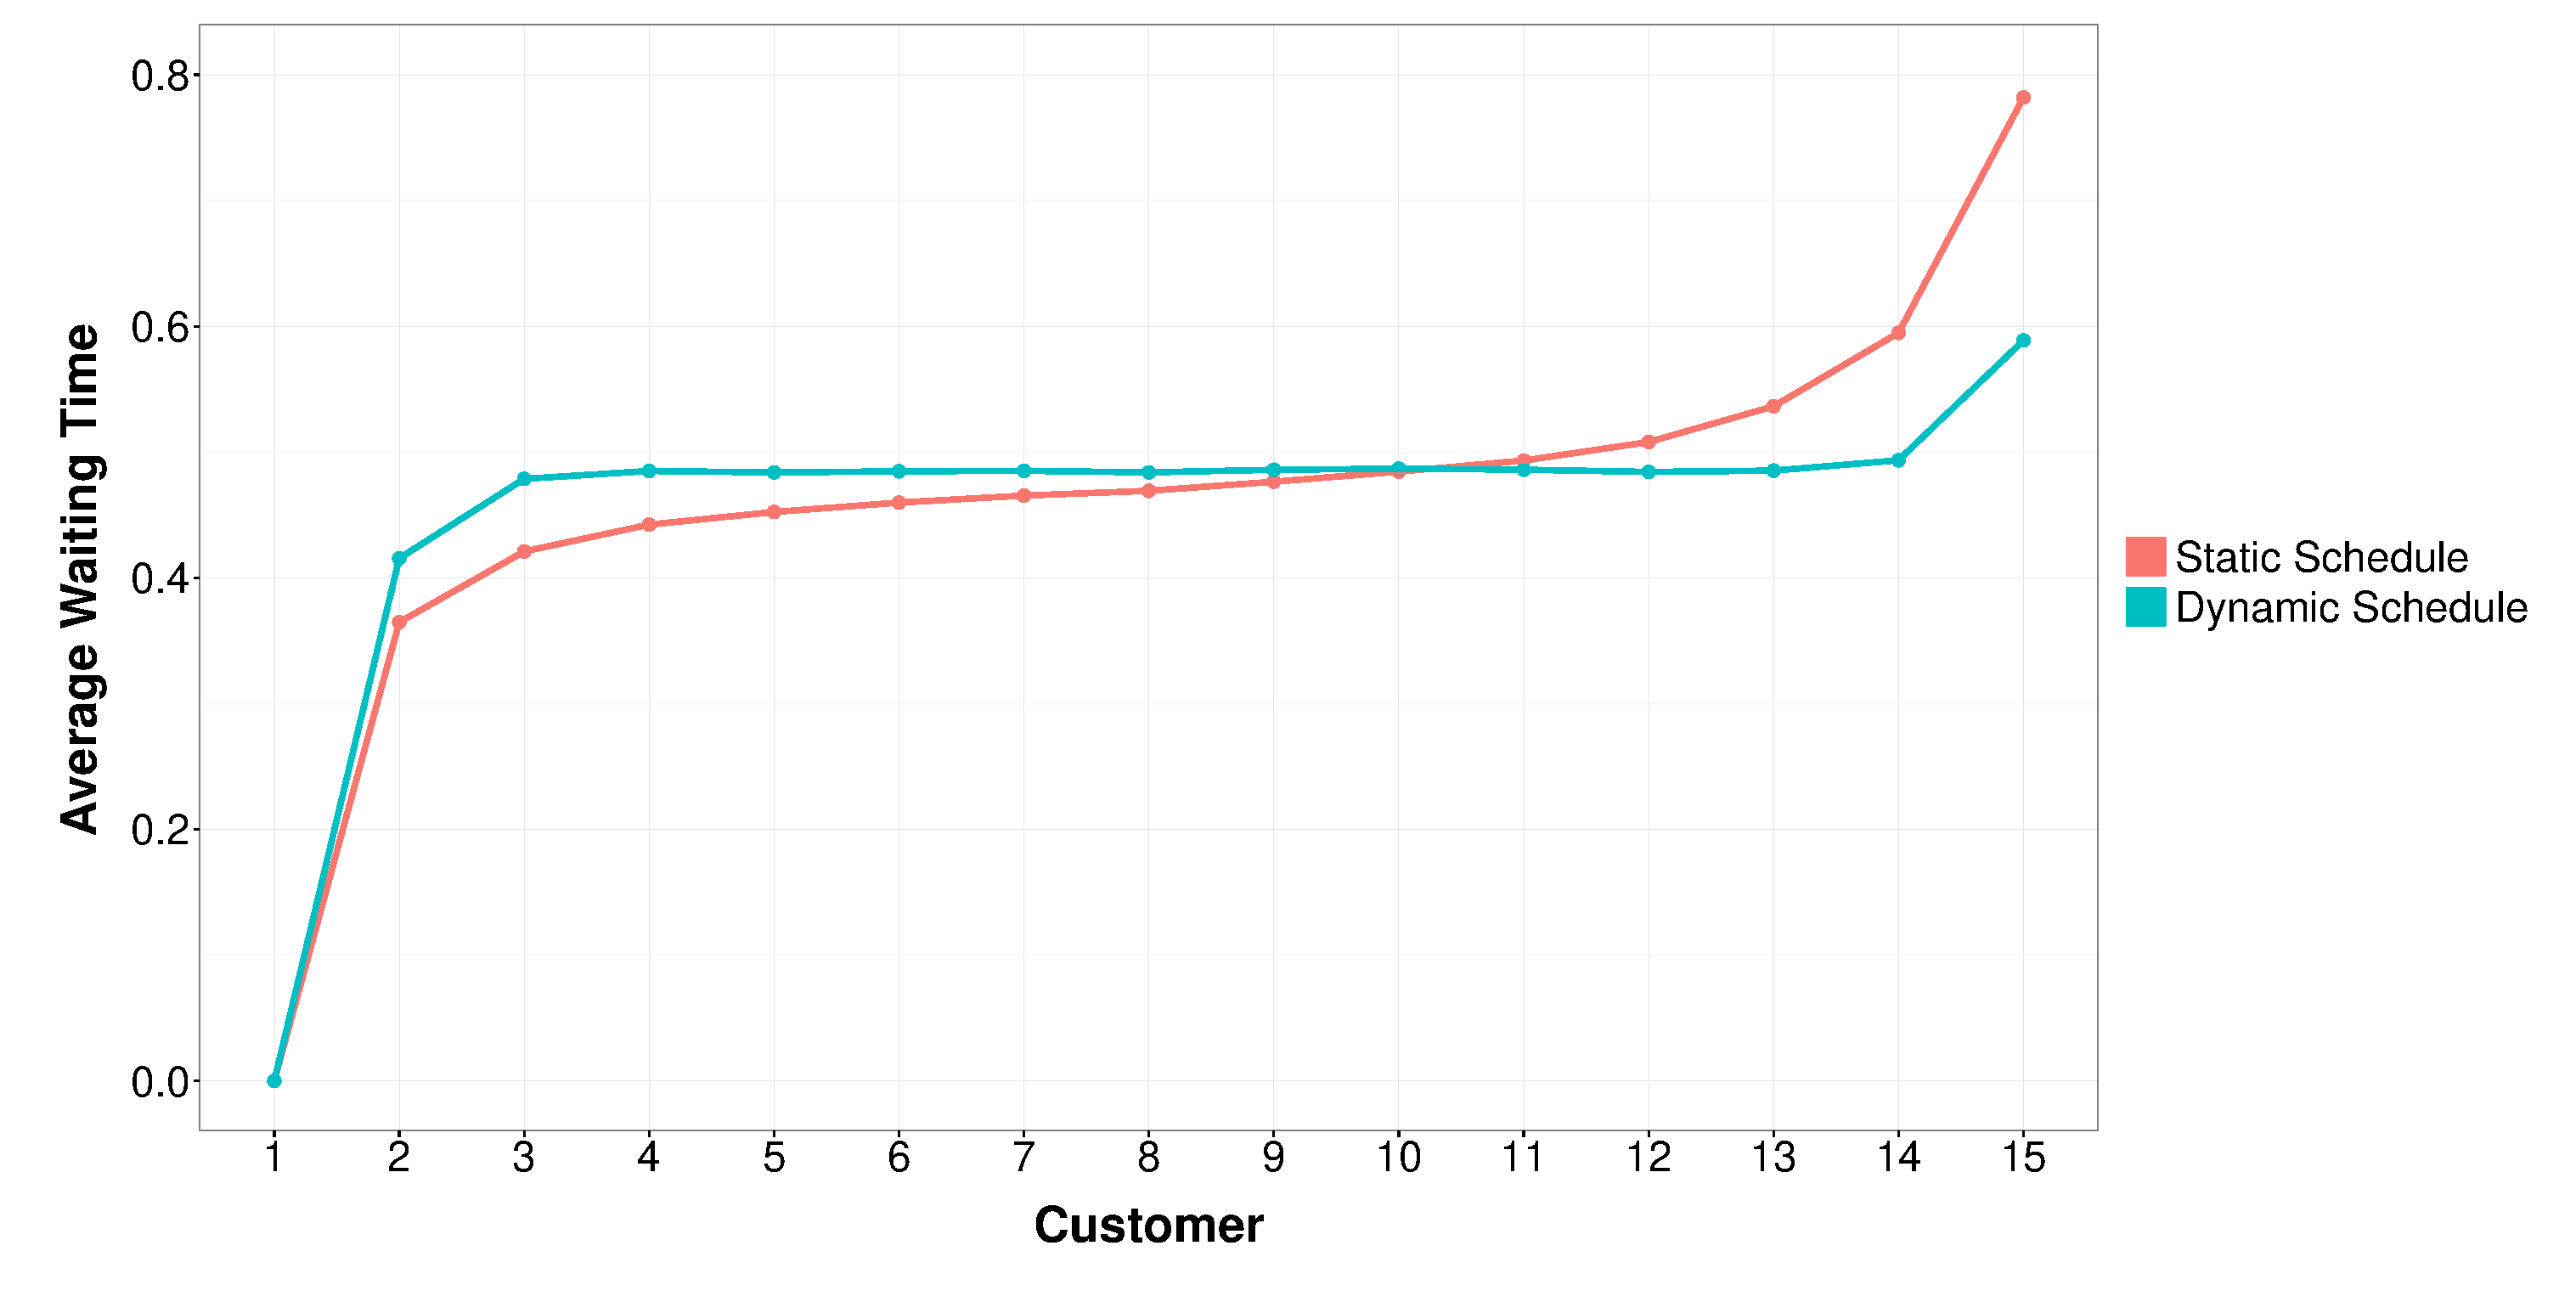
\includegraphics[width = 0.85\textwidth]{WT_Line_Avg.eps}
	\caption{Plot of the average waiting time for each of the $15$ customers for each schedule where $\mu = 1$ and $\gamma = \frac{c_{S}}{c_{S} + c_{W}} = 0.5$.}
	\label{fig:Avg_Wait_Position}
\end{figure}

In both schedules, the average waiting time of the first customer is $0$ as they are served immediately. The first few customers wait longer on average in the dynamic schedule than the static schedule. In contrast, the later few customers tend to wait significantly longer in the static schedule. From customer $3$ up to customer $14$, their average waiting times are increases for the static schedule, but approximately constant in the dynamic schedule. It appears that the dynamic schedule is significantly `fairer' and able to spread the waiting time more evenly amongst the customers. The static schedule tends to favour the earlier customers.

Intuitively, customers prefer schedules where they are served immediately and do not have to wait. Figure~\ref{fig:No_Wait_Position} plots the proportion of runs where each customer does not have to wait.
\begin{figure}[htb]
	\centering
	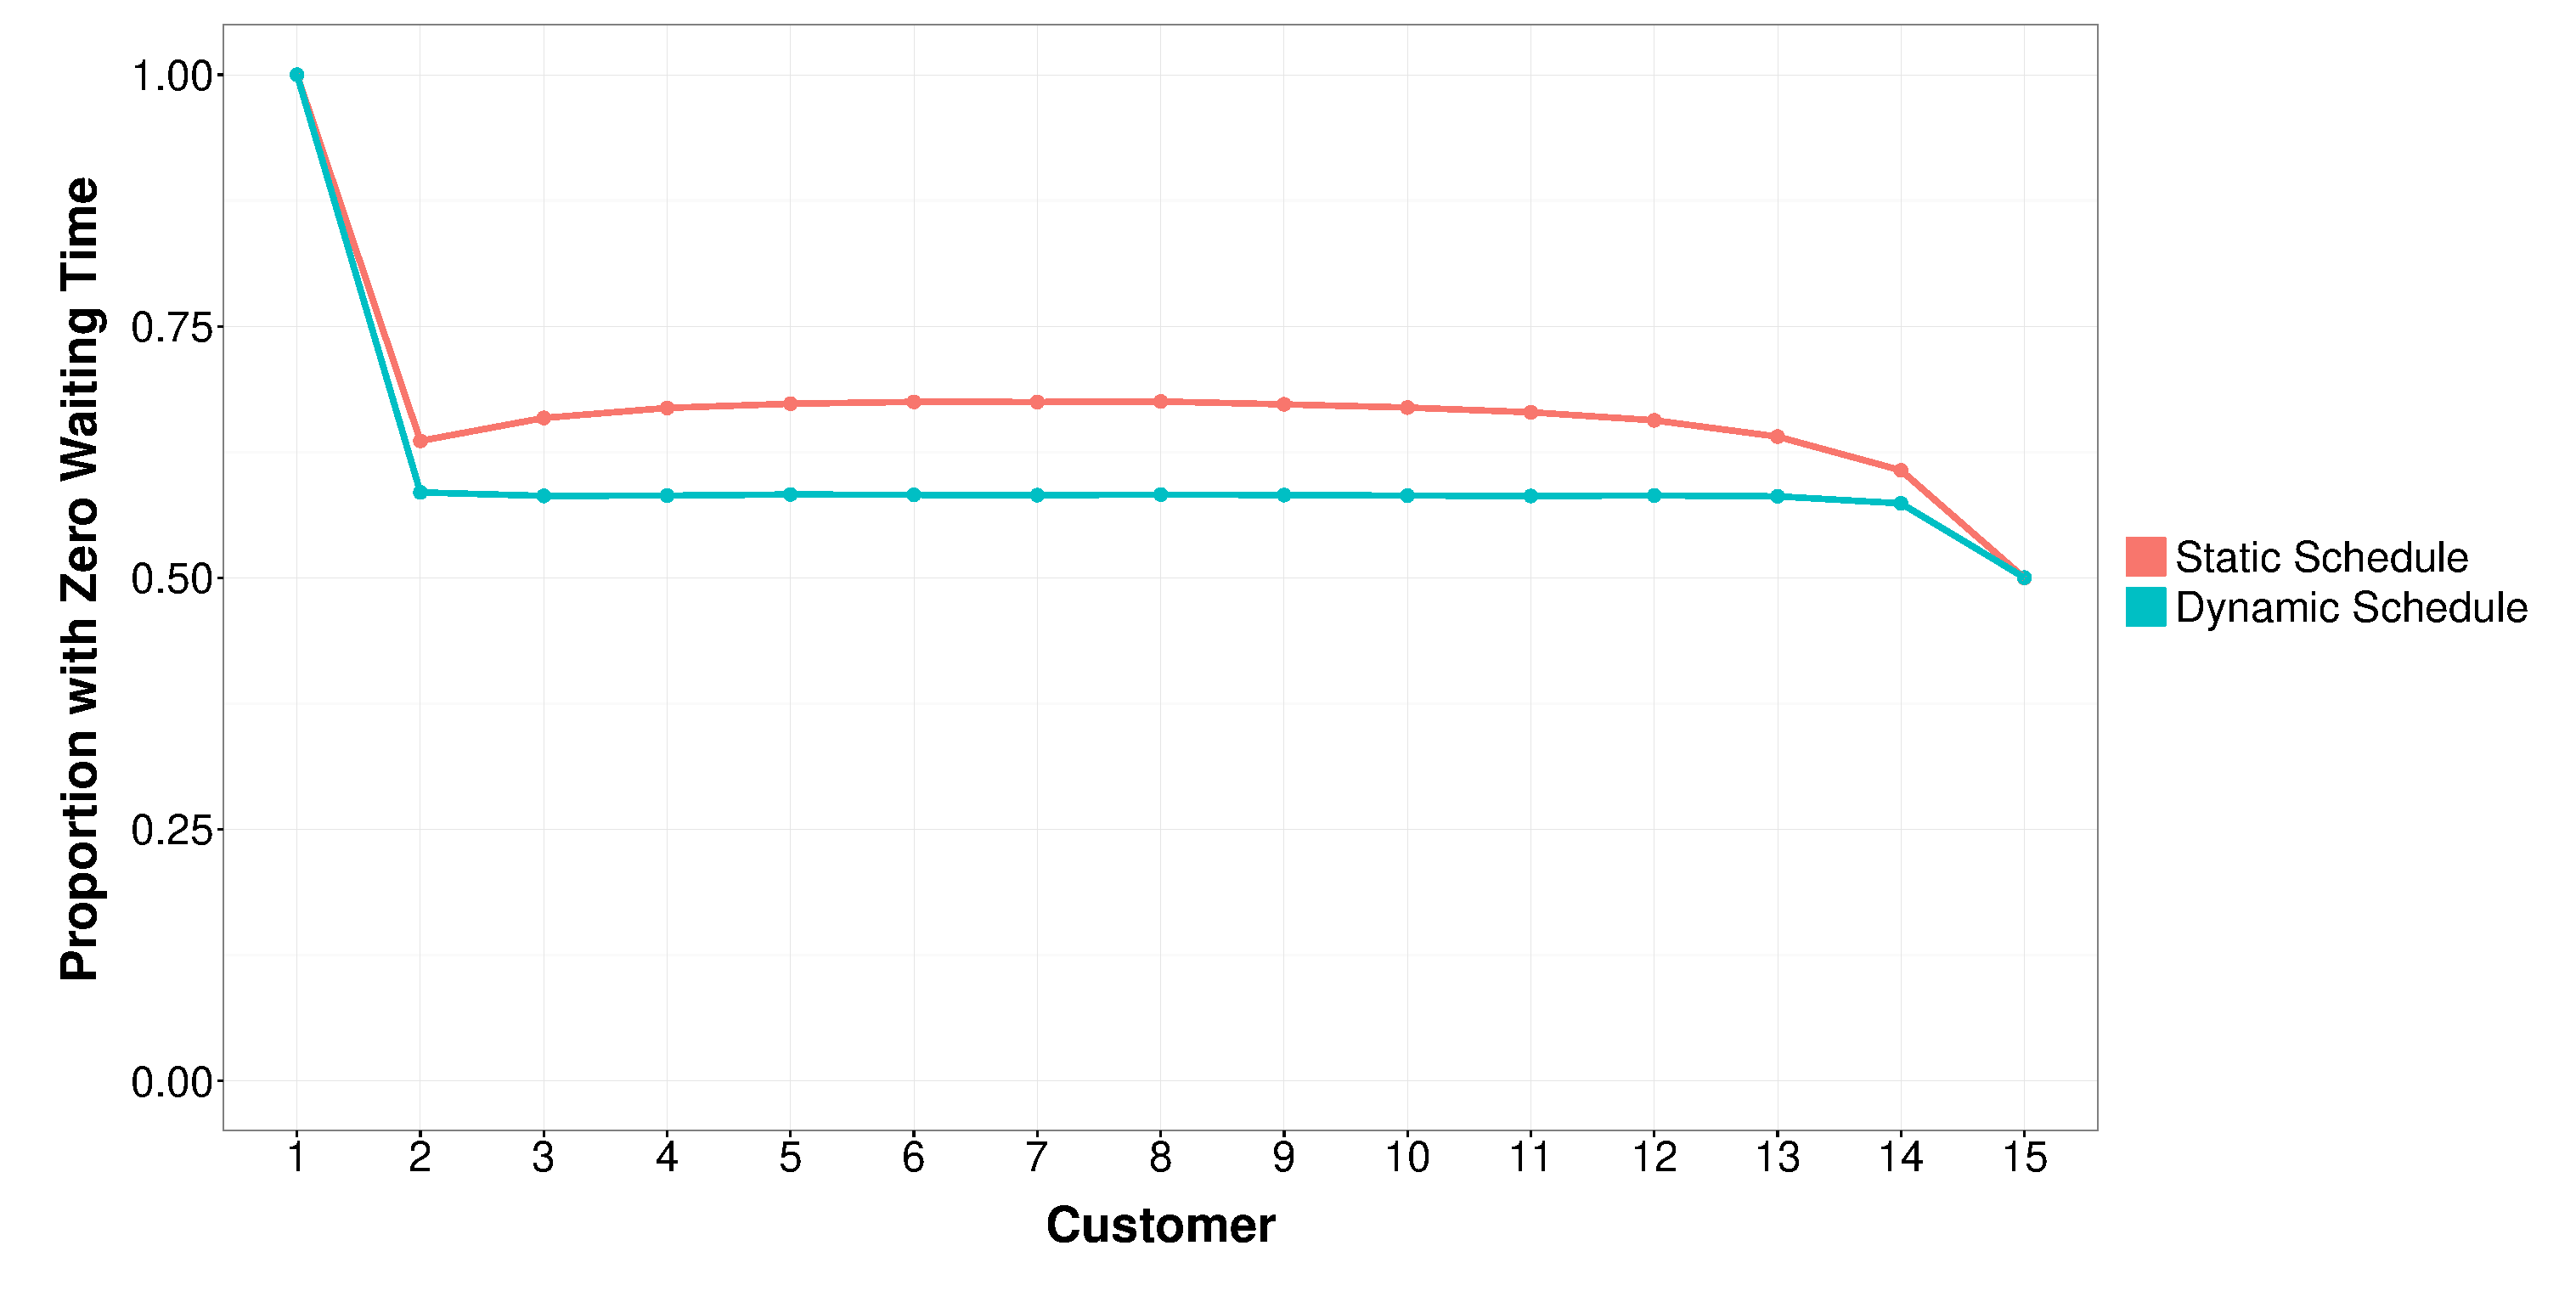
\includegraphics[width = 0.85\textwidth]{WT_Line_Prop.eps}
	\caption{Plot of the proportion of all runs where the customer does not wait for each of the $15$ customers for each schedule where $\mu = 1$ and $\gamma = \frac{c_{S}}{c_{S} + c_{W}} = 0.5$.}
	\label{fig:No_Wait_Position}
\end{figure}

In both schedules, the first customer never waits and is served immediately in $100 \%$ of the runs. The dynamic schedule again appears to be fairer. The proportion of runs with no waiting appears to be constant for all except the first and last customers. All customers (except the first and last) are served immediately a greater proportion of the time in the static schedule than the dynamic schedule. While this is advantageous for the customers, it leads to a longer idle time of the server and thus a longer server availability time.

\section{Server Availability Time}
The schedules do not only attempt to minimise customer waiting time, but they also attempt to minimise the total server availability time. Figure~\ref{fig:Two_Server} plots the histograms of the total server availability times of the static and dynamic schedules for each run of the simulation.
\begin{figure}[htb]
	\centering
	\begin{subfigure}[t]{0.45\textwidth}
		\centering
		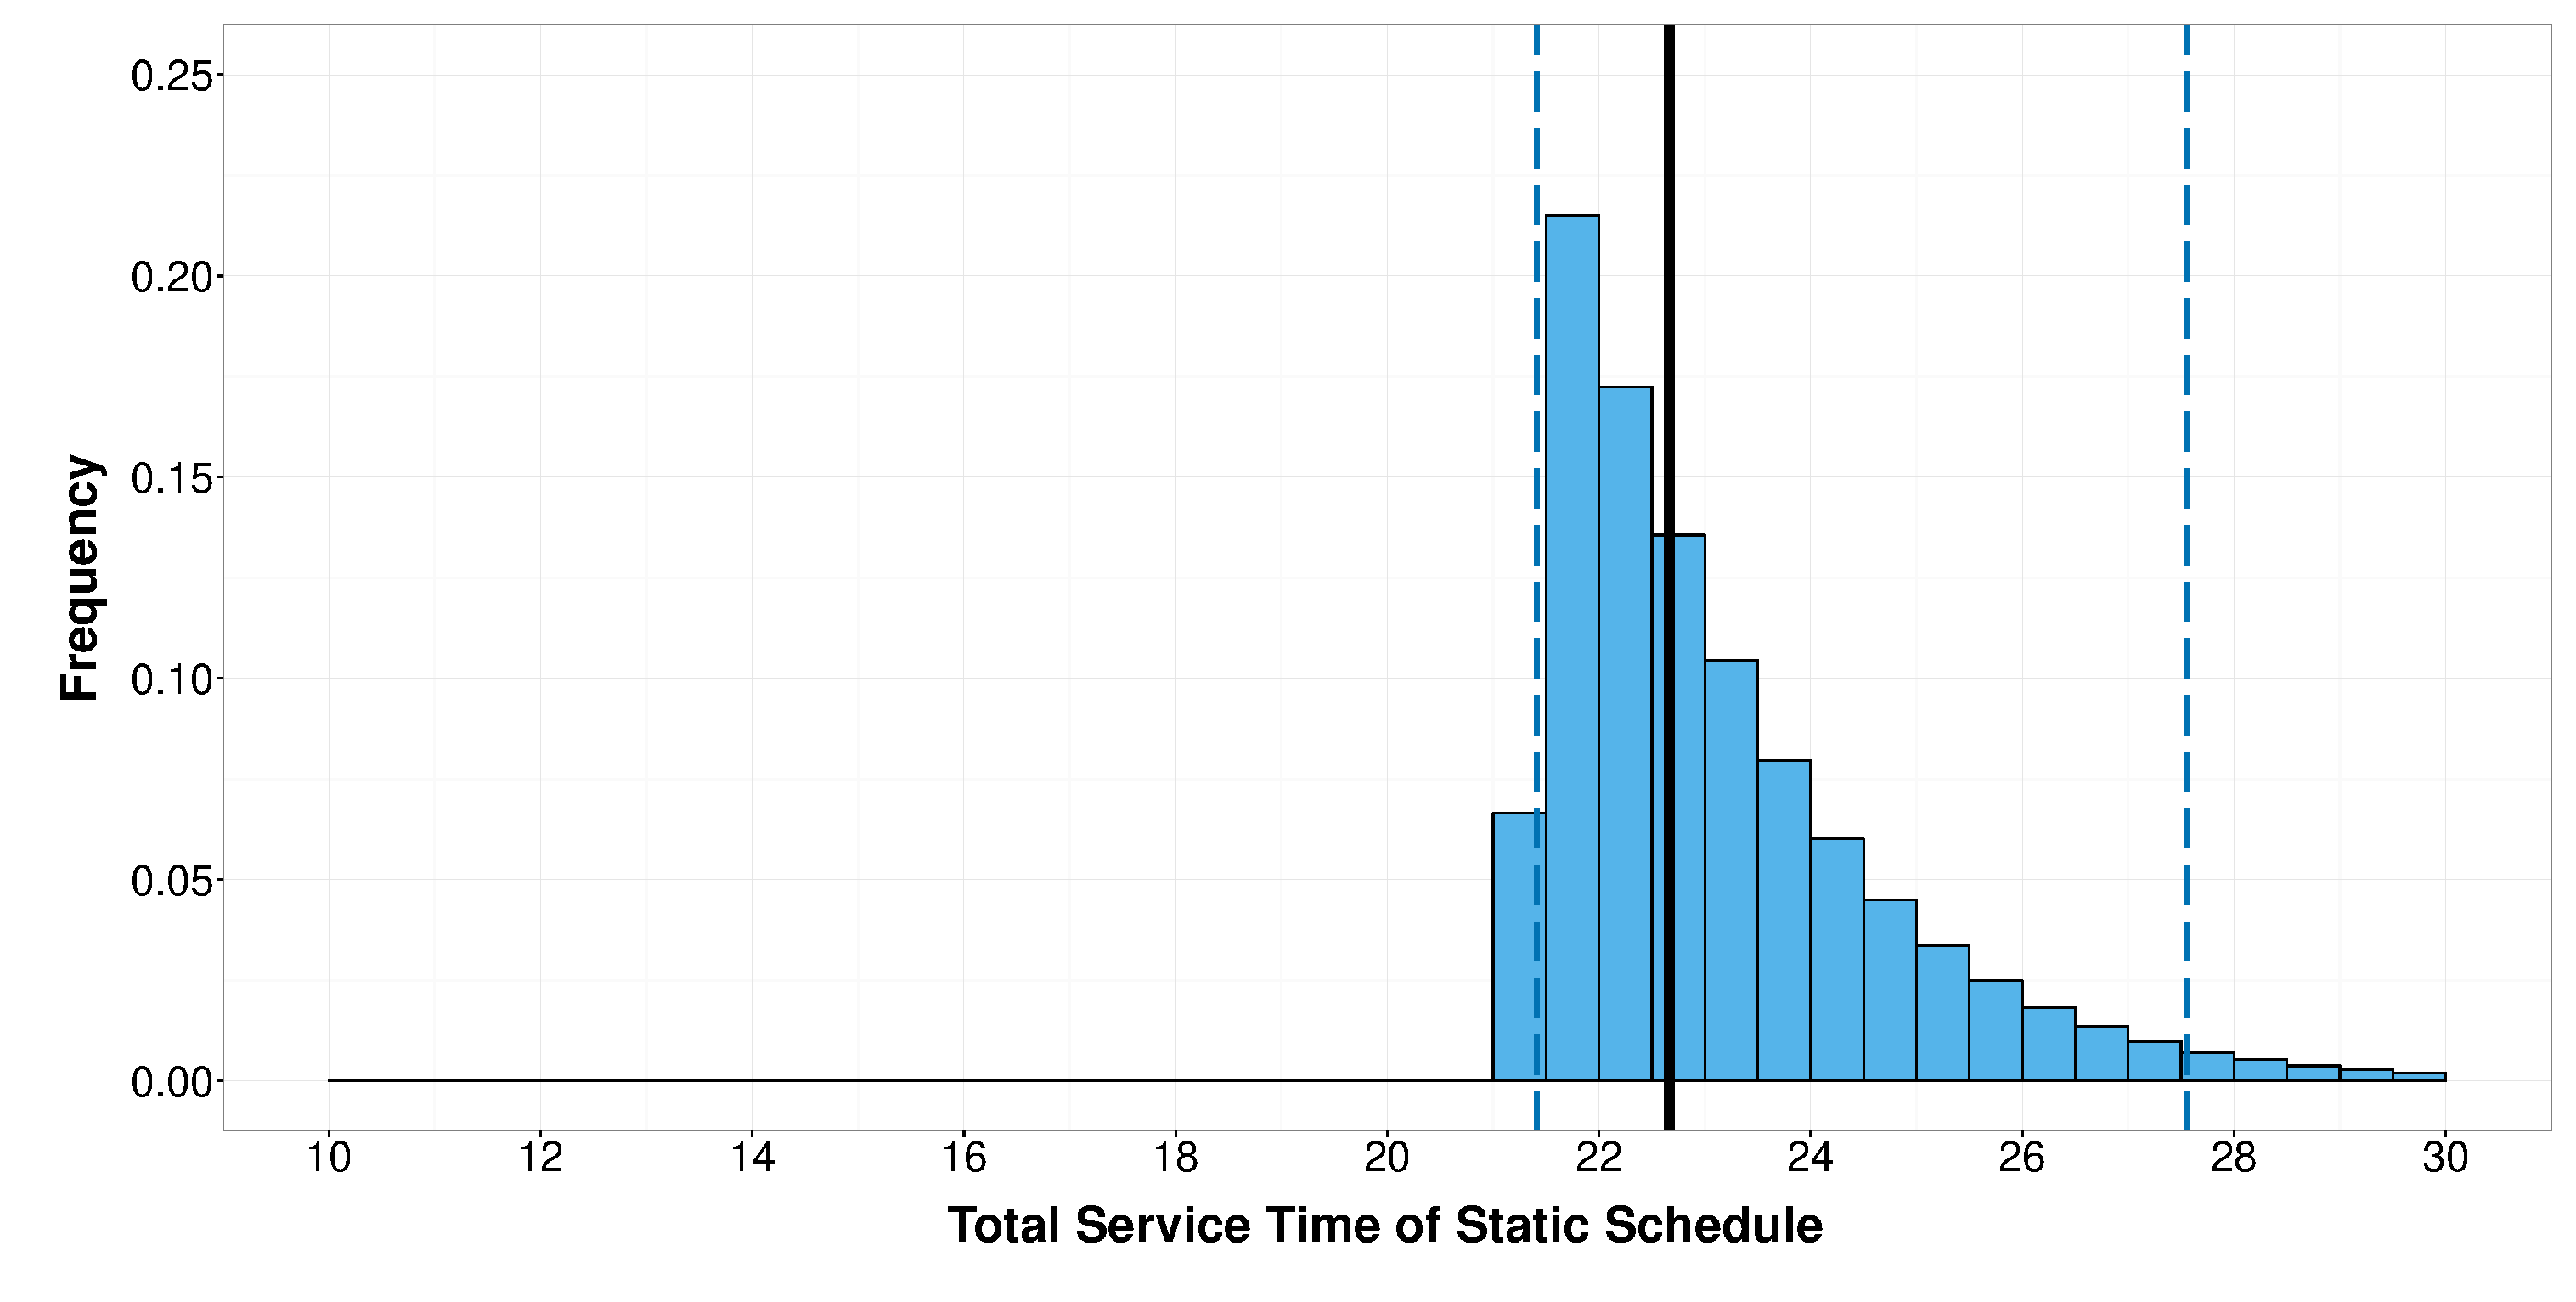
\includegraphics[width=\textwidth]{TST_Hist_Static.eps}
		\caption{}
	\end{subfigure}
	\begin{subfigure}[t]{0.45\textwidth}
		\centering
		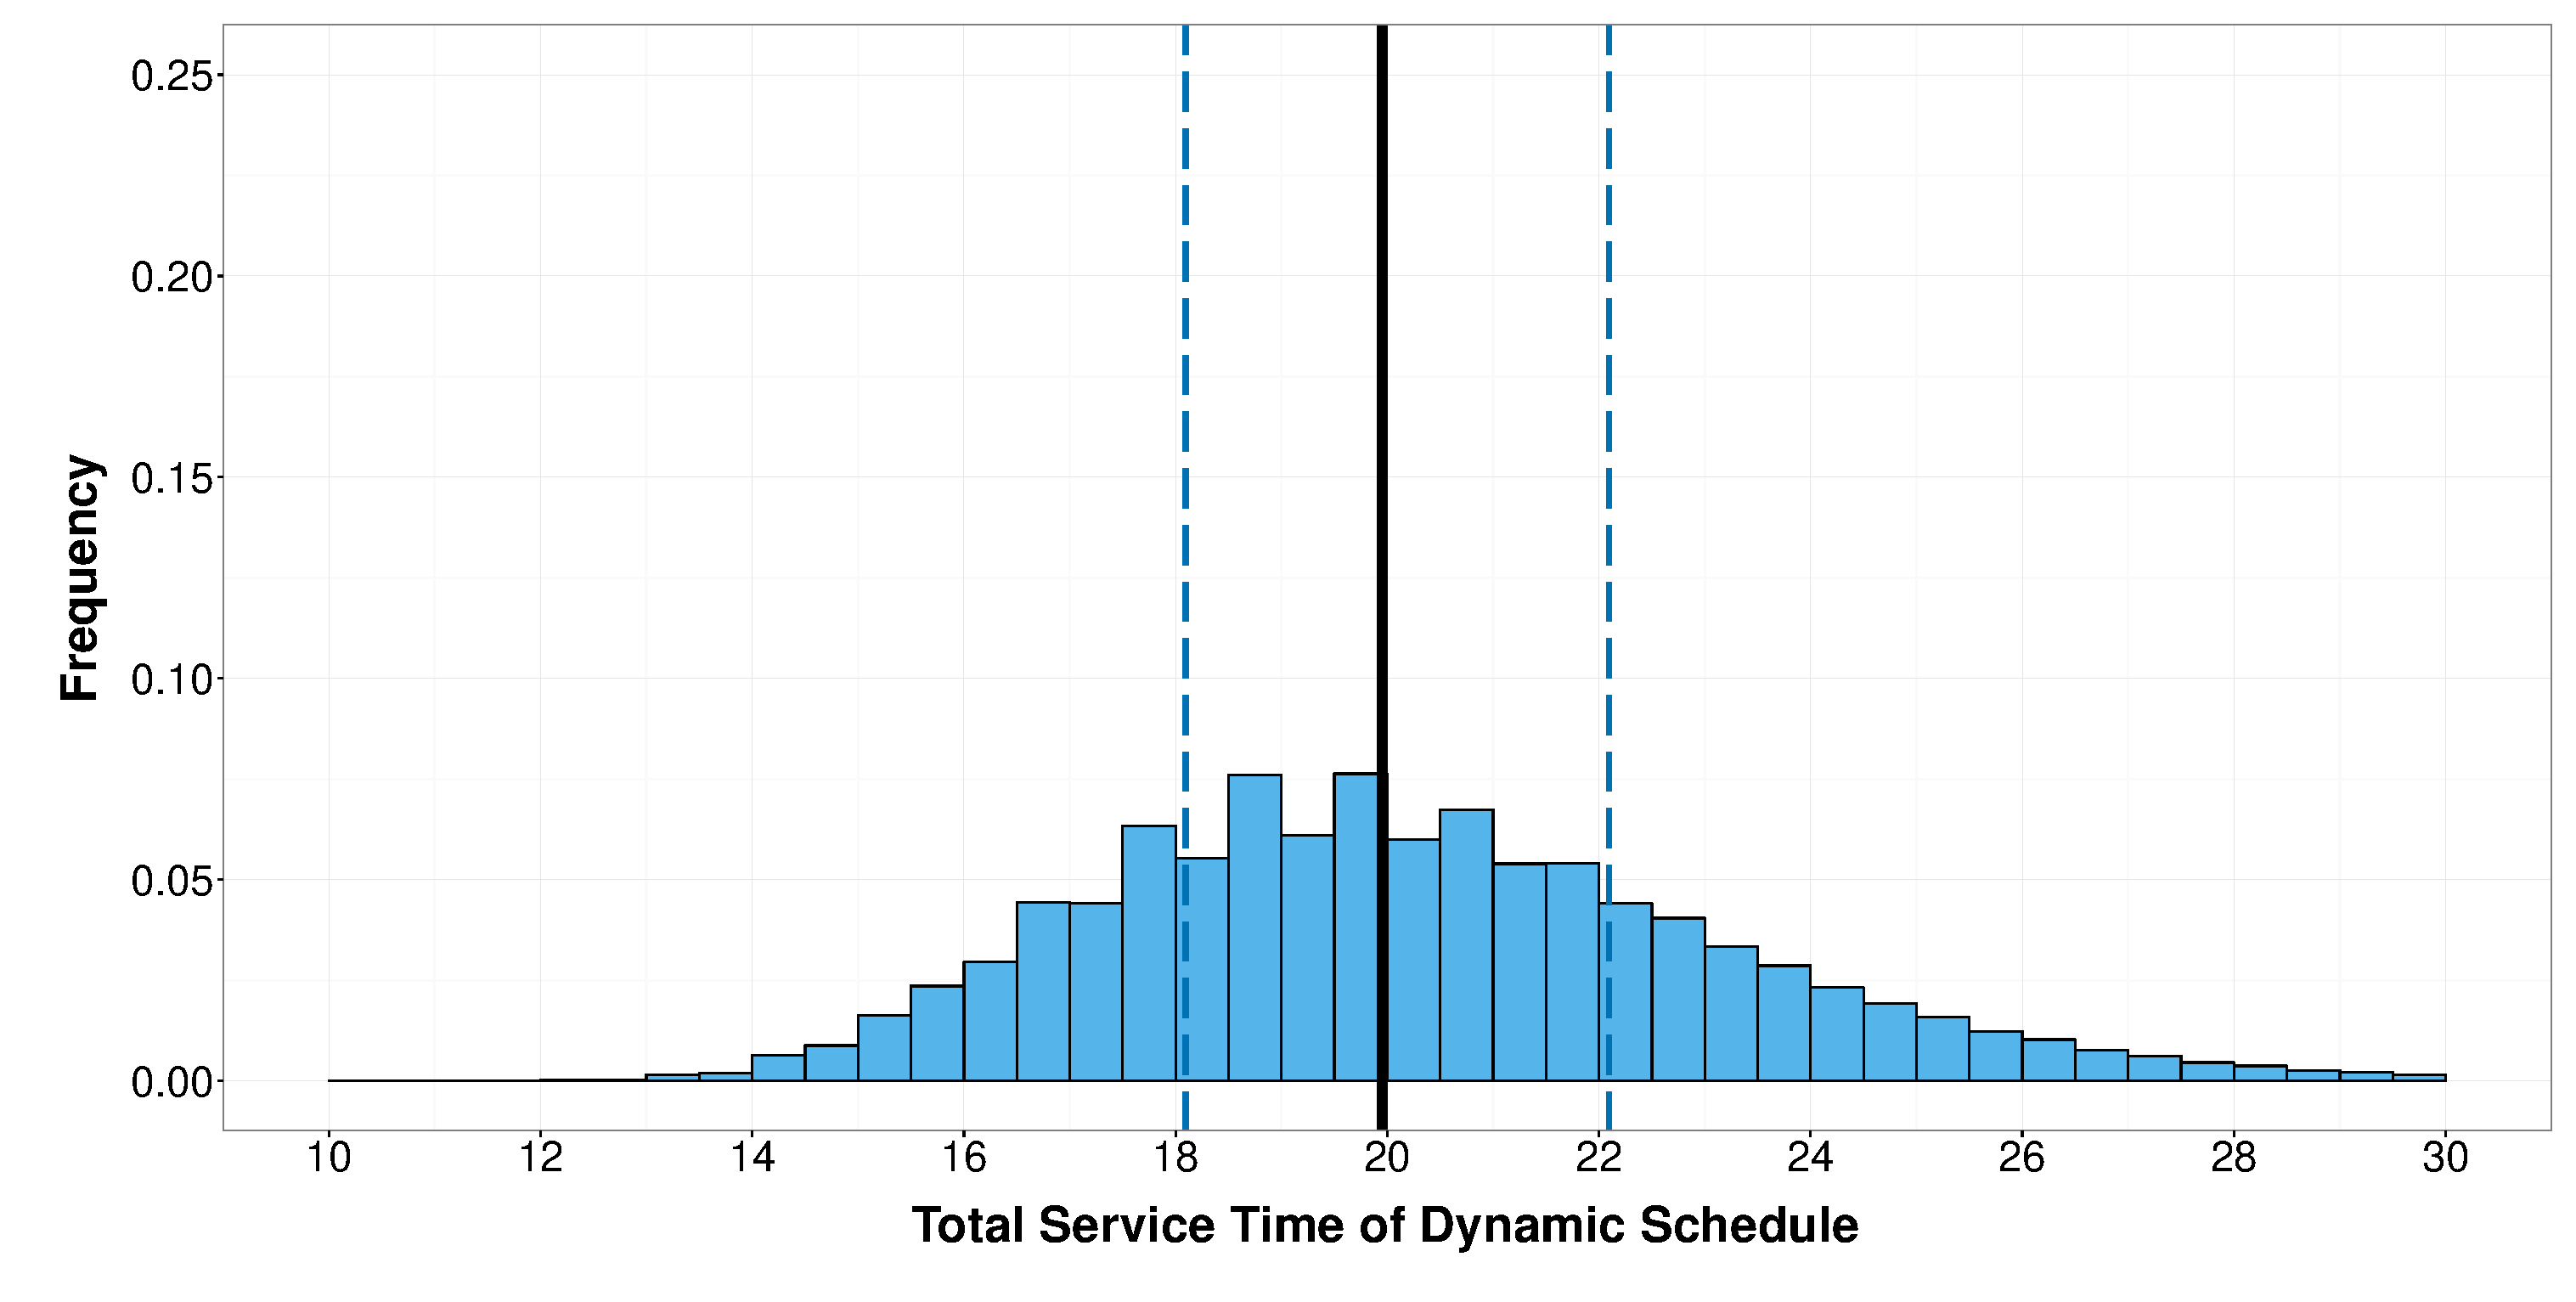
\includegraphics[width=\textwidth]{TST_Hist_Dynamic.eps}
		\caption{}
	\end{subfigure}
	\caption{Histogram plot of the total server availability times for the static (a) and dynamic (b) schedules for each simulation run where $\mu = 1$ and $\gamma = \frac{c_{S}}{c_{S} + c_{W}} = 0.5$. The black vertical line indicates the median and the blue dashes lines indicate the upper and lower quartiles.}
	\label{fig:Two_Server}
\end{figure}

The median total server availability time is $22.66$ for the static schedule and $19.95$ for the dynamic schedule. While the customer waiting time appears to be generally similar for both schedules, the dynamic schedule appears to attain its lower expected cost due to its lower total server availability time. This agrees with the idea from Chapter~\ref{chap:Comparison} that the expected percentage cost saving is lowest where $\gamma = \frac{c_{S}}{c_{S} + c_{W}}$ is small. If the per unit time of the server availability time is small then the dynamic schedule's ability to reduce the total server availability time is less effective at reduce the cost of the schedule.

Moreover, the minimum total server availability time is significantly lower in the case of the dynamic schedule. The minimum total server availability time is $21.37$ for the static schedule and $12.11$ for the dynamic schedule. This is especially surprising as both minimums occur in the same run of the simulation. The static schedule is significantly limited by the fixed arrival of the last customer at $21.36$ time units. The dynamic schedule is able to adjust the customer arrival times and attain a broader range of total server availability times that are lower on average.

\chapter{Conclusion}
The goal of this thesis was to derive methods for determining the optimal customer arrival times in a single-server queue with punctual customers. In Chapter~\ref{chap:Static}, we derived a similar method to \citet{Pegden} for determining the optimal static schedule. In Chapter~\ref{chap:Dynamic}, we derived an iterative procedure for determining the optimal dynamic schedule. This procedure determines the optimal arrival time of the next customer given the number of customers still to be scheduled and the number of customers currently in the system. In both schedules, the optimal schedule minimises a linear combination of the expected total customer waiting time and the expected server availability time.

In Chapter~\ref{chap:Static}, we were able to derive algebraic expressions for the optimal policy for schedules with less than three customers. As expected, the interarrival time between the first two customers decreases as the server availability cost increases. In addition, we found numerical solutions for the case of scheduling $15$ customers. We observed the dome-shape, which is a commonly observed property of static schedules. The optimal interarrival times increase for the initial few customers, remain constant for the majority of customers, and decrease for the final few customers.

In Chapter~\ref{chap:Dynamic}, we derived algebraic expressions for the optimal dynamic schedule where there are less than three customers. These dynamic schedules exactly match the optimal static schedules found in Chapter~\ref{chap:Static}. For more than two customers, the optimal dynamic schedule consists of the optimal policies at each of the possible states during service.

We considered the case of scheduling $15$ customers using a dynamic schedule. We found that the optimal interarrival time of the next customer appears to only depend on the number currently in the system provided that it is not the final customer being scheduled. If this hypothesis was proved in the general case, then it would have several potential benefits. First, it would be significantly easier to apply such a schedule in practice as the scheduler is only required to know a few optimal policies. Moreover, it would be more efficient to compute the optimal dynamic schedule as it would involve solving for a smaller number of unknown variables. However, more work is required to confirm this hypothesis.

In Chapter~\ref{chap:Comparison}, we compared the expected cost of the two schedules. As expected, the static schedule never has a smaller expected cost than the dynamic schedule. However, we found that the expected cost difference only appears to be noticeable when scheduling more than five customers. The expected percentage cost saving increases as the number of customers to be scheduled increases, but at a decreasing rate. For scheduling $15$ customers, the expected percentage cost saving is generally between $5$ and $10\%$. From our results, it does not appear that the expected percentage cost saving would ever exceed $15\%$.

In Chapter~\ref{chap:Simulation}, we used simulation to get a fuller understanding of the differences between the two schedules. The dynamic schedule is able to adapt during service, and is thus less prone to simulation runs with extremely high cost. The dynamic schedule generally schedules customers to arrive earlier than the static schedule. Customers thus often have longer waiting times in the dynamic schedule. However, the dynamic schedule appears to be fairer as the average waiting time is approximately constant for the majority of the customers. The dynamic schedule appears to attain its lower expected cost due to its considerably lower server availability time. For $15$ customers where $\gamma = 0.5$, the median server availability time is $12 \%$ lower for the dynamic schedule.

The results presented in this thesis suggest that the dynamic schedule can often significantly outperform the static schedule. Models that ignore the potential ability to reschedule arrival times appear to be too restrictive. However, this work should be extended to more clearly understand how the rescheduling ability should be included.

A highly beneficial extension of the dynamic schedule presented in Chapter~\ref{chap:Dynamic} would include the idea of a minimum notice period. In many situations, customers are not able to arrive immediately. The dynamic schedule would be more applicable if it could include a minimum value on the scheduled interarrival times. For the minimum notice period to be properly included in the schedule, the schedule must have the ability to schedule multiple customers at once rather than needing to schedule the customers one-by-one.

Other extensions on the schedules prevented in this thesis would involve adjustments to the objective function. Many papers include the server's idle time in the objective. Both the objective function for the static schedule in Chapter~\ref{chap:Static} and the expected transition cost in Chapter~\ref{chap:Dynamic} can be easily adjusted to include the cost of the server's idle time.

Another extension on the objective function could include the cost of overtime. The service could have a desired finish time, and there is a (high) cost if the service exceeds this time. This extension would be beneficial to real world services. However, applying it requires knowledge of this desired finish time parameter, which is likely heavily dependent on the specific service under consideration.

\appendix

\chapter{Dynamic Schedule Derivation}

\section{Transition Probability}
This is a derivation of the probability $p_{a} (k, j)$. This is the probability that there are $k - (j - 1)$ departures from a queue over $a$ time units assuming the queue initially has $k$ customers and no new arrivals. The customer service times are iid exponential random variables with mean $\mu$.

The probabililty is most easily derived on a case by case basis.

\subsection{Case 1 $k = 0$}
The first case is that the queue initially has no customers. For any $a \geq 0$, there will be no departures from the queue over $a$ time units.
\begin{equation}
	p_{a} (k, j) = \mathbbm{1} (j = 1)
\end{equation}

\subsection{Case 2 $k \geq 1, j = 1$}
Denote the service times of the $k$ customers as $S_{1}, \ldots, S_{k}$. If $j = 1$, then $p_{a} (k, j)$ is the probability of $k$ departures from the queue over $a$ time units. The sum $\sum_{i = 1}^{k} S_{i}$ has an Erlang distribution with cdf $F (a; k)$.
\begin{equation}
	p_{a} (k, j) = \mathbb{P} \left( \sum_{i = 1}^{k} S_{i} \leq a \right) = F (a; k)
\end{equation}

\subsection{Case 3 $k \geq 2, 2 \leq j \leq k$}
For $2 \leq j \leq k$, $p_{a} (k, j)$ is the probability that the total service time of the first $k - (j - 1)$ customers is less that $a$, and the total service time of the first $k - (j - 1) + 1$ customers is greater than $a$.
\begin{equation}
	\begin{split}
		p_{a} (k, j)
		& = \mathbb{P} \left( \sum_{i = 1}^{k - (j - 1)} S_{i} \leq a, \sum_{i = 1}^{k - (j - 1) + 1} S_{i} > a \right) \\
		& = \mathbb{P} \left( \sum_{i = 1}^{k - (j - 1)} S_{i} \leq a, S_{k - (j - 1) + 1} > a - \sum_{i = 1}^{k - (j - 1)} S_{i} \right) \\
	\end{split}
\end{equation}

Condition the probability on $\sum_{i = 1}^{k - (j - 1)} S_{i} = z$, which has pdf $f (z; k - (j - 1))$ and integrate over all possible values of $z$.
\begin{equation}
	\begin{split}
		p_{a} (k, j)
		& = \int_{0}^{\infty} \mathbb{P} (z \leq a, S_{k - (j - 1) + 1} > a - z) f \big( z; k - (j - 1) \big) \ d z \\
		& = \int_{0}^{a} \mathbb{P} (S_{k - (j - 1) + 1} > a - z) f \big( z; k - (j - 1) \big) \ d z \\
		& = \frac{1}{(k - j)!} \left( \frac{1}{\mu} \right)^{k - j + 1} \mathrm{e}^{\frac{- a}{\mu}} \int_{0}^{a} z^{k - j} \ d z \\
		& = \frac{1}{(k - j + 1)!} \left( \frac{a}{\mu} \right)^{k - j + 1} \mathrm{e}^{\frac{- a}{\mu}} \\
		& = F (a; k - j + 1) - F (a; k - j + 2)
	\end{split}
\end{equation}

\subsection{Case 4 $k \geq 1, j = k + 1$}
For $j = k + 1$, $p_{a} (k, j)$ is the probability that the service time of the first customer is longer than $a$ time units.
\begin{equation}
	p_{a} (k, j) = \mathbb{P} (S_{1} > a) = 1 - \mathbb{P} (S_{1} \leq a) = 1 - F (a; 1)
\end{equation}

\subsection{All Other Cases}
All other cases have zero probability.
\begin{equation}
	p_{a} (k, j) = 0
\end{equation}

\subsection{Summary}
These results can be summarised as:
\begin{equation}
	p_{a} (k, j) = \begin{cases}
		\mathbbm{1} (j = 1) & \text{for $k = 0$} \\
		F (a; k) & \text{for $k \geq 1, j = 1$} \\
		F (a; k - j + 1) - F (a; k - j + 2) & \text{for $k \geq 2, 2 \leq j \leq k$} \\
		1 - F (a; 1) & \text{for $k \geq 1, j = (k + 1)$} \\
		0 & \text{otherwise}
	\end{cases}
\end{equation}

\section{Expected Transition Cost}
This is a derivation of the expected cost $R_{a} (k, j)$. This is the expected cost of transitioning from the state $(n, k)$ to the state $(n - 1, j)$ over $a$ time units if the next customer is scheduled to arrive in $a$ time units. The expected cost is a linear combination of the expected total customers' waiting times and the expected server availability time. The per unit time costs $c_{W}$ and $c_{S}$ are defined as in Chapter~\ref{chap:Static}.

In a similar way to the transition probability, the cost is most easily derived on a case by case basis.

\subsection{Case 1 $k \in \{ 0, 1 \}$}
The first case is that the system initially has either no customers or only a single customer. In this case, no customers are waiting during the transition, so the total customers waiting time is zero. The only cost is the cost of expected server availability time during the transition. The server is available for the entire transition, so the server availability time is $a$.
\begin{equation}
	R_{a} (k, j) = c_{S} a
\end{equation}

\subsection{Case 2 $k \geq 2, j = 1$}
If $j = 1$, then all $k$ customers finish service during the transition. This implies that $\displaystyle \sum_{n = 1}^{k} S_{n} \leq a$. The total customers' waiting time is a linear combination of the service times given that the sum of all $k$ is smaller than $k$. The server is still available for the entire transition, so the server availability time is $a$.
\begin{equation}
	\begin{split}
		R_{a} (k, j) & = c_{W} \sum_{i = 2}^{k} \mathbb{E} \left[ \sum_{l = 1}^{i - 1} S_{l} \ \vline \ \sum_{n = 1}^{k} S_{n} \leq a \right] + c_{S} a \\
		& = c_{W} \mathbb{E} \left[ S_{1} \ \vline \ \sum_{n = 1}^{k} S_{n} \leq a \right] \sum_{i = 2}^{k} (i - 1) + c_{S} a \\
		& = c_{W} \frac{k (k - 1)}{2} \mathbb{E} \left[ S_{1} \ \vline \ \sum_{n = 1}^{k} S_{n} \leq a \right] + c_{S} a \\
		& = c_{W} \frac{(k - 1)}{2} \mathbb{E} \left[ \sum_{n = 1}^{k} S_{n} \ \vline \ \sum_{n = 1}^{k} S_{n} \leq a \right] + c_{S} a \\
	\end{split}
\end{equation}

The term $\displaystyle \mathbb{E} \left[ \sum_{n = 1}^{k} S_{n} \ \vline \ \sum_{n = 1}^{k} S_{n} \leq a \right]$ is one of the conditional expectations defined in Chapter~\ref{chap:Dynamic}.
\begin{equation}
	R_{a} (k, j) = c_{W} \frac{G (a; k) (k - 1)}{2} + c_{S} a
\end{equation}

\subsection{Case 3 $k \geq 2, 2 \leq j \leq k$}
For $2 \leq j \leq k$, then the first $k - (j - 1)$ customers finish service during the transition, but customer $k - (j - 1) + 1$ does not. This implies that $\displaystyle \sum_{n = 1}^{k - (j - 1)} S_{n} \leq a$ and $\displaystyle \sum_{n = 1}^{k - (j - 1) + 1} S_{n} > a$. The last $j - 2$ customers wait for the entire transition. In addition, the server is available for the entire transition.
\begin{equation}
	\begin{split}
		R_{a} (k, j)
		= & \ c_{W} \sum_{i = 2}^{k - (j - 2)} \mathbb{E} \left[ \sum_{l = 1}^{i - 1} S_{l} \ \vline \ \sum_{n = 1}^{k - (j - 1)} S_{n} \leq a, \sum_{n = 1}^{k - (j - 1) + 1} S_{n} > a \right] \\
		& + c_{W} \sum_{i = 1}^{j - 2} a + c_{S} a \\
		= & \ c_{W} \mathbb{E} \left[ S_{1} \ \vline \ \sum_{n = 1}^{k - (j - 1)} S_{n} \leq a, \sum_{n = 1}^{k - (j - 1) + 1} S_{n} > a \right] \sum_{i = 2}^{k - (j - 2)} (i - 1) \\
		& + c_{W} a (j - 2) + c_{S} a \\
		= & \ c_{W} \frac{ \big[ k - (j - 1) \big] \big[ k - (j - 2) \big]}{2} \mathbb{E} \left[ S_{1} \ \vline \ \sum_{n = 1}^{k - (j - 1)} S_{n} \leq a, \sum_{n = 1}^{k - (j - 1) + 1} S_{n} > a \right] \\
		& + c_{W} a (j - 2) + c_{S} a \\
		= & \ c_{W} \frac{ \big[ k - (j - 2) \big]}{2} \mathbb{E} \left[ \sum_{n = 1}^{k - (j - 1)} S_{n} \ \vline \ \sum_{n = 1}^{k - (j - 1)} S_{n} \leq a, \sum_{n = 1}^{k - (j - 1) + 1} S_{n} > a \right] \\
		& + c_{W} a (j - 2) + c_{S} a \\
	\end{split}
\end{equation}

The term $\displaystyle \mathbb{E} \left[ \sum_{n = 1}^{k - (j - 1)} S_{n} \ \vline \ \sum_{n = 1}^{k - (j - 1)} S_{n} \leq a, \sum_{n = 1}^{k - (j - 1) + 1} S_{n} > a \right]$ is another of the conditional expectations defined in Chapter~\ref{chap:Dynamic}.
\begin{equation}
	\begin{split}
		R_{a} (k, j)
		= & \ c_{W} \left[ \frac{H \big( a; k - (j - 1) \big) \big[ k - (j - 2) \big]}{2} + a (j - 2) \right] + c_{S} a \\
		= & \ c_{W} \left[ \frac{a \big[ k - (j - 1) \big]}{2} + a (j - 2) \right] + c_{S} a \\
		= & \ c_{W} \frac{a (k + j - 3)}{2} + c_{S} a
	\end{split}
\end{equation}

\subsection{Case 4 $k \geq 2, j = (k + 1)$}
For $j = k + 1$, no customers finish service during the transition. All customers except the first customer wait for the entire transition. The server is available for the entire transition.
\begin{equation}
	R_{a} (k, j) = c_{W} \sum_{i = 1}^{k - 1} a + c_{S} a = c_{W} a (k - 1) + c_{S} a
\end{equation}

\subsection{Summary}
In order to compare the dynamic schedule with the static schedule, need to scale these costs by dividing by $(c_{S} + c_{W})$ and defining $\gamma = \frac{c_{S}}{c_{S} + c_{W}}$. These results can be summarised as:
\begin{equation}
	R_{a} (k, j) = \begin{cases}
		\gamma a & \text{for $k \in \{ 0, 1 \}$} \\
		(1 - \gamma) \frac{G (a; k) (k - 1)}{2} + \gamma a & \text{for $k \geq 2, j = 1$} \\
		(1 - \gamma) \frac{a (k + j - 3)}{2} + \gamma a & \text{for $k \geq 2, 2 \leq j \leq k + 1$} \\
	\end{cases}
\end{equation}



















































\printbibliography

\end{document}